\documentclass[]{book}
\usepackage{lmodern}
\usepackage{amssymb,amsmath}
\usepackage{ifxetex,ifluatex}
\usepackage{fixltx2e} % provides \textsubscript
\ifnum 0\ifxetex 1\fi\ifluatex 1\fi=0 % if pdftex
  \usepackage[T1]{fontenc}
  \usepackage[utf8]{inputenc}
\else % if luatex or xelatex
  \ifxetex
    \usepackage{mathspec}
  \else
    \usepackage{fontspec}
  \fi
  \defaultfontfeatures{Ligatures=TeX,Scale=MatchLowercase}
\fi
% use upquote if available, for straight quotes in verbatim environments
\IfFileExists{upquote.sty}{\usepackage{upquote}}{}
% use microtype if available
\IfFileExists{microtype.sty}{%
\usepackage[]{microtype}
\UseMicrotypeSet[protrusion]{basicmath} % disable protrusion for tt fonts
}{}
\PassOptionsToPackage{hyphens}{url} % url is loaded by hyperref
\usepackage[unicode=true]{hyperref}
\hypersetup{
            pdftitle={Data Network Dashboards},
            pdfauthor={This document is currently under construction},
            pdfborder={0 0 0},
            breaklinks=true}
\urlstyle{same}  % don't use monospace font for urls
\usepackage{natbib}
\bibliographystyle{apalike}
\usepackage{color}
\usepackage{fancyvrb}
\newcommand{\VerbBar}{|}
\newcommand{\VERB}{\Verb[commandchars=\\\{\}]}
\DefineVerbatimEnvironment{Highlighting}{Verbatim}{commandchars=\\\{\}}
% Add ',fontsize=\small' for more characters per line
\usepackage{framed}
\definecolor{shadecolor}{RGB}{248,248,248}
\newenvironment{Shaded}{\begin{snugshade}}{\end{snugshade}}
\newcommand{\KeywordTok}[1]{\textcolor[rgb]{0.13,0.29,0.53}{\textbf{#1}}}
\newcommand{\DataTypeTok}[1]{\textcolor[rgb]{0.13,0.29,0.53}{#1}}
\newcommand{\DecValTok}[1]{\textcolor[rgb]{0.00,0.00,0.81}{#1}}
\newcommand{\BaseNTok}[1]{\textcolor[rgb]{0.00,0.00,0.81}{#1}}
\newcommand{\FloatTok}[1]{\textcolor[rgb]{0.00,0.00,0.81}{#1}}
\newcommand{\ConstantTok}[1]{\textcolor[rgb]{0.00,0.00,0.00}{#1}}
\newcommand{\CharTok}[1]{\textcolor[rgb]{0.31,0.60,0.02}{#1}}
\newcommand{\SpecialCharTok}[1]{\textcolor[rgb]{0.00,0.00,0.00}{#1}}
\newcommand{\StringTok}[1]{\textcolor[rgb]{0.31,0.60,0.02}{#1}}
\newcommand{\VerbatimStringTok}[1]{\textcolor[rgb]{0.31,0.60,0.02}{#1}}
\newcommand{\SpecialStringTok}[1]{\textcolor[rgb]{0.31,0.60,0.02}{#1}}
\newcommand{\ImportTok}[1]{#1}
\newcommand{\CommentTok}[1]{\textcolor[rgb]{0.56,0.35,0.01}{\textit{#1}}}
\newcommand{\DocumentationTok}[1]{\textcolor[rgb]{0.56,0.35,0.01}{\textbf{\textit{#1}}}}
\newcommand{\AnnotationTok}[1]{\textcolor[rgb]{0.56,0.35,0.01}{\textbf{\textit{#1}}}}
\newcommand{\CommentVarTok}[1]{\textcolor[rgb]{0.56,0.35,0.01}{\textbf{\textit{#1}}}}
\newcommand{\OtherTok}[1]{\textcolor[rgb]{0.56,0.35,0.01}{#1}}
\newcommand{\FunctionTok}[1]{\textcolor[rgb]{0.00,0.00,0.00}{#1}}
\newcommand{\VariableTok}[1]{\textcolor[rgb]{0.00,0.00,0.00}{#1}}
\newcommand{\ControlFlowTok}[1]{\textcolor[rgb]{0.13,0.29,0.53}{\textbf{#1}}}
\newcommand{\OperatorTok}[1]{\textcolor[rgb]{0.81,0.36,0.00}{\textbf{#1}}}
\newcommand{\BuiltInTok}[1]{#1}
\newcommand{\ExtensionTok}[1]{#1}
\newcommand{\PreprocessorTok}[1]{\textcolor[rgb]{0.56,0.35,0.01}{\textit{#1}}}
\newcommand{\AttributeTok}[1]{\textcolor[rgb]{0.77,0.63,0.00}{#1}}
\newcommand{\RegionMarkerTok}[1]{#1}
\newcommand{\InformationTok}[1]{\textcolor[rgb]{0.56,0.35,0.01}{\textbf{\textit{#1}}}}
\newcommand{\WarningTok}[1]{\textcolor[rgb]{0.56,0.35,0.01}{\textbf{\textit{#1}}}}
\newcommand{\AlertTok}[1]{\textcolor[rgb]{0.94,0.16,0.16}{#1}}
\newcommand{\ErrorTok}[1]{\textcolor[rgb]{0.64,0.00,0.00}{\textbf{#1}}}
\newcommand{\NormalTok}[1]{#1}
\usepackage{longtable,booktabs}
% Fix footnotes in tables (requires footnote package)
\IfFileExists{footnote.sty}{\usepackage{footnote}\makesavenoteenv{long table}}{}
\usepackage{graphicx,grffile}
\makeatletter
\def\maxwidth{\ifdim\Gin@nat@width>\linewidth\linewidth\else\Gin@nat@width\fi}
\def\maxheight{\ifdim\Gin@nat@height>\textheight\textheight\else\Gin@nat@height\fi}
\makeatother
% Scale images if necessary, so that they will not overflow the page
% margins by default, and it is still possible to overwrite the defaults
% using explicit options in \includegraphics[width, height, ...]{}
\setkeys{Gin}{width=\maxwidth,height=\maxheight,keepaspectratio}
\IfFileExists{parskip.sty}{%
\usepackage{parskip}
}{% else
\setlength{\parindent}{0pt}
\setlength{\parskip}{6pt plus 2pt minus 1pt}
}
\setlength{\emergencystretch}{3em}  % prevent overfull lines
\providecommand{\tightlist}{%
  \setlength{\itemsep}{0pt}\setlength{\parskip}{0pt}}
\setcounter{secnumdepth}{5}
% Redefines (sub)paragraphs to behave more like sections
\ifx\paragraph\undefined\else
\let\oldparagraph\paragraph
\renewcommand{\paragraph}[1]{\oldparagraph{#1}\mbox{}}
\fi
\ifx\subparagraph\undefined\else
\let\oldsubparagraph\subparagraph
\renewcommand{\subparagraph}[1]{\oldsubparagraph{#1}\mbox{}}
\fi

% set default figure placement to htbp
\makeatletter
\def\fps@figure{htbp}
\makeatother

\usepackage{booktabs}
\usepackage{amsthm}
\makeatletter
\def\thm@space@setup{%
  \thm@preskip=8pt plus 2pt minus 4pt
  \thm@postskip=\thm@preskip
}
\makeatother

\title{Data Network Dashboards}
\author{This document is currently under construction}
\date{2020-03-05}

\begin{document}
\maketitle

{
\setcounter{tocdepth}{1}
\tableofcontents
}
\chapter*{Preface}\label{preface}
\addcontentsline{toc}{chapter}{Preface}

Automated Characterization of Health Information at Large-scale
Longitudinal Evidence Systems (ACHILLES) is a profiling tool developed
by the OHDSI community to provide descriptive statistics of databases
standardized to the OMOP Common Data Model. These characteristics are
presented graphically in the ATLAS tool. However, this solution does not
allow for database comparison across the data network. The Data Network
Dashboards aggregates ACHILLES results files from databases in the
network and displays the descriptive statistics through graphical
dashboards. This tool is helpful to gain insight in the growth of the
data network and is useful for the selection of databases for specific
research questions. In the software demonstration we show a first
version of this tool that will be further developed in EHDEN in close
collaboration with all our stakeholders, including OHDSI.

\section*{Contributors}\label{contributors}
\addcontentsline{toc}{section}{Contributors}

To develop this tool, EHDEN organized a hack-a-thon (Aveiro, December
2-3, 2019), where we defined and implemented a series of charts and
dashboards containing the most relevant information about the OMOP CDM
databases. The team involved in this task were composed by the following
members:

\begin{itemize}
\tightlist
\item
  João Rafael Almeida\textsuperscript{1}
\item
  André Pedrosa\textsuperscript{1}
\item
  Peter R. Rijnbeek\textsuperscript{2}
\item
  Marcel de Wilde\textsuperscript{2}
\item
  Michel Van Speybroeck\textsuperscript{3}
\item
  Maxim Moinat\textsuperscript{4}
\item
  Pedro Freire\textsuperscript{1}
\item
  Alina Trifan\textsuperscript{1}
\item
  Sérgio Matos\textsuperscript{1}
\item
  José Luís Oliveira\textsuperscript{1}
\end{itemize}

1 - Institute of Electronics and Informatics Engineering of Aveiro,
Department of Electronics and Telecommunication, University of Aveiro,
Aveiro, Portugal

2 - Erasmus MC, Rotterdam, Netherlands

3 - Janssen Pharmaceutica NV, Beerse, Belgium

4 - The Hyve, Utrecht, Netherlands

\section*{Considerations}\label{considerations}
\addcontentsline{toc}{section}{Considerations}

This manual was written to be a guide for a clean installation of this
system with all the dashboards that we defined during the project. The
first chapter describes the goal of the system and the second how to
install the system. The remaining chapters are dedicated to the
dashboards, in which chapters describes one dashboard and all its
charts. To simplify the representation of the dashboard's layout, we
used similar schemas as it is presented in Figure
\ref{fig:dashboardsLayout}. The white box is the dashboard and the
inside boxes are charts. The colour changes in relation to the type of
chart.

\begin{figure}
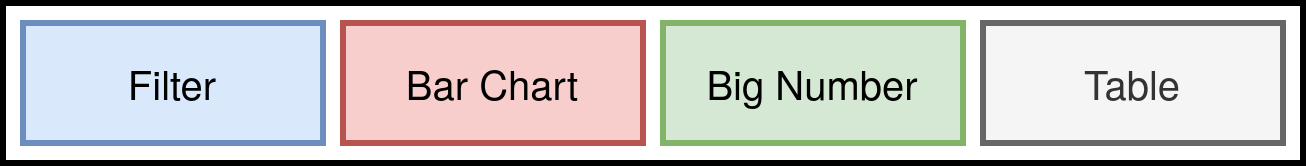
\includegraphics[width=1\linewidth]{images/dashboardsLayout} \caption{Example of a dashboards tool presenting the databases available in the network (simulated data)}\label{fig:dashboardsLayout}
\end{figure}

\section*{License}\label{license}
\addcontentsline{toc}{section}{License}

The system is open-source and this manual was written in
\href{https://rmarkdown.rstudio.com}{RMarkdown} using the
\href{https://bookdown.org}{bookdown} package.

\section*{Acknowledges}\label{acknowledges}
\addcontentsline{toc}{section}{Acknowledges}

This work has been conducted in the context of EHDEN, a project that
receives funding from the European Union's Horizon 2020 and EFPIA
through IMI2 Joint Undertaking initiative, under grant agreement No
806968.

\chapter{Introduction}\label{introduction}

The OHDSI research network has been growing steadily which results in an
increasing number of healthcare databases standardized to the OMOP CDM
format. The OHDSI community created the ACHILLES tool (Automated
Characterization of Health Information at Large-scale Longitudinal
Exploration System) to characterize those databases. The results are
available to the data custodian in their local ATLAS tool and helps them
to gain insights in their data and helps in assessing the feasibility of
a particular research questions.

ACHILLES was designed to extract the metadata from a single database,
which by itself does not allow the comparison with the remaining
databases in the network. However, we believe there is even more value
in sharing this information with others to enable network research in a
Data Network Dashboard.

\section{Data Network Dashboard}\label{data-network-dashboard}

The European Health Data and Evidence Network (EHDEN) project therefore
designed a Data Network Dashboard tool, a web application to aggregate
information from distributed OMOP CDM databases. It uses the ACHILLES
results files to construct graphical dashboards and enables database
comparison (Figure \ref{fig:cdmBI}). The tool is built on Apache
Superset, which is an open-source enterprise-ready business intelligence
web application that can provide powerful and fully customizable
graphical representations of data. Achilles results can be uploaded
through the EHDEN Database Catalogue using the dashboards plugin but can
also be directly uploaded in the tool. Figure 1. Example of a dashboards
tool presenting age and gender distributions (simulated data).

\begin{figure}
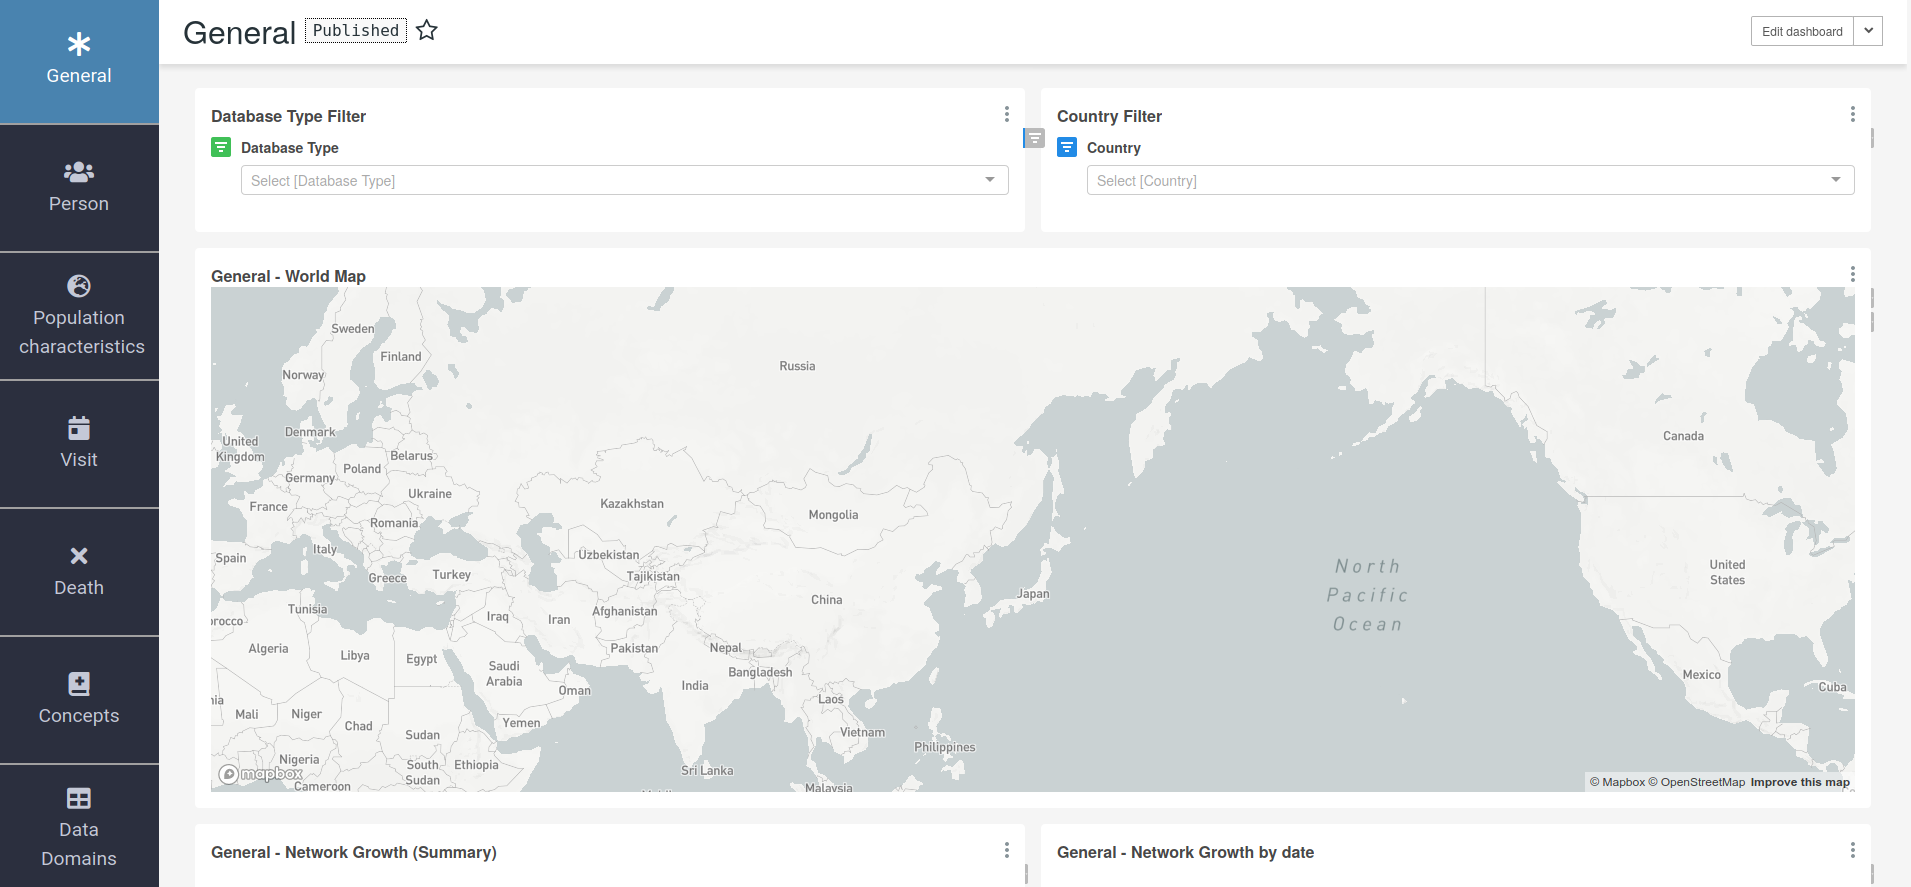
\includegraphics[width=1\linewidth]{images/cdmBI} \caption{Example of a dashboards tool presenting the databases available in the network (simulated data)}\label{fig:cdmBI}
\end{figure}

In this tools, we defined and implemented a series of charts and
dashboards containing the most relevant information about the databases,
such as:

\begin{itemize}
\tightlist
\item
  \textbf{General}: dashboards that shows the databases types per
  country, the distribution of data source types, the growth of the
  Network including the number of database and the number of patients in
  the databases over time;
\item
  \textbf{Person}: representing the number of patients per country, age
  distribution at first observation, year of birth distribution and
  normalized gender distribution;
\item
  \textbf{Population characteristics}: dashboard with the cumulative
  patient time, persons with continuous observation per month, and the
  start and end dates of those periods;
\item
  \textbf{Visit}: chart to compare the number and type of visit
  occurrence records;
\item
  \textbf{Death}: information about the number of death records by
  month, and the patient age at time of death;
\item
  \textbf{Concepts}: bubble chart which shows the number of patients and
  records per concept over the databases;
\item
  \textbf{Data domains}: heat map visualization of the major data
  domains in each database.
\end{itemize}

\chapter{Installation}\label{installation}

NOTE: This instructions are outdated

Make sure that you have docker and docker-compose installed in your
machine. Then, please follow these steps:

\begin{itemize}
\item
  Please enter in the `'docker'' directory and create your \texttt{.env}
  file here, using \texttt{.env-example} as reference. For local
  installation, you can just copy the \texttt{.env-example} content to a
  new file. Note: In case of port errors in the next steps, the problem
  could be related to a port already in use by your system that you
  defined here and it is busy, chose other.
\item
  Tip the following commands in the command line:

  \begin{enumerate}
  \def\labelenumi{\arabic{enumi}.}
  \item
    Clone the Apache Superset repository:

\begin{verbatim}
git clone https://github.com/apache/incubator-superset
 ../superset
cp ../superset/contrib/docker/superset_config.py ../superset
\end{verbatim}
  \item
    Init the Apache Superset (This creates a user, so it is necessary to
    interact with the console):

\begin{verbatim}
docker-compose run --rm superset ./docker-init.sh
\end{verbatim}
  \item
    Init the Dashboard Layout (This creates a user, so it is necessary
    to interact with the console):

\begin{verbatim}
docker-compose run --rm dashboard_viewer ./docker-init.sh
\end{verbatim}
  \item
    Finally, bring up the containers

\begin{verbatim}
docker-compose up -d
\end{verbatim}
  \end{enumerate}
\end{itemize}

To check if everything is ok, please wait 2 minutes and tip
\texttt{docker\ ps} and the following containers need to be running:

\begin{verbatim}
... 0.0.0.0:8088->8088/tcp   dashboard_viewer_superset_1
... 0.0.0.0:8000->8000/tcp   dashboard_viewer_dashboard_viewer_1
... 0.0.0.0:6379->6379/tcp   dashboard_viewer_redis_1
... 5432/tcp                 dashboard_viewer_postgres_1
\end{verbatim}

Now, you have a clean setup running in your machine. To try the
application using synthetic data, please continue to follow the steps in
the `'Demo'' section.

\section{Insert Concepts}\label{insert-concepts}

The concepts table are not in the repository due to its dimension.
Therefore, to insert this table in the installation, you should perform
the following steps:

\begin{enumerate}
\def\labelenumi{\arabic{enumi}.}
\item
  Download concept.csv file from here (todo)
\item
  Copy the file to the /tmp directory inside of the postgres container

\begin{Shaded}
\begin{Highlighting}[]
\ExtensionTok{docker}\NormalTok{ cp concept.csv dashboard_viewer_postgres_1:/tmp/}
\end{Highlighting}
\end{Shaded}
\item
  Enter in the dashboard\_viewer\_postgres\_1 container:

\begin{Shaded}
\begin{Highlighting}[]
\ExtensionTok{docker}\NormalTok{ exec -it dashboard_viewer_postgres_1 bash}
\end{Highlighting}
\end{Shaded}
\item
  Enter in the achilles database:

\begin{verbatim}
psql achilles
\end{verbatim}
\item
  Create the table in the database using this command:

\begin{Shaded}
\begin{Highlighting}[]
    \KeywordTok{CREATE} \KeywordTok{TABLE}\NormalTok{ concept (}
\NormalTok{      concept_id         }\DataTypeTok{INTEGER}        \KeywordTok{NOT} \KeywordTok{NULL}\NormalTok{,}
\NormalTok{      concept_name       }\DataTypeTok{VARCHAR}\NormalTok{(}\DecValTok{255}\NormalTok{)   }\KeywordTok{NOT} \KeywordTok{NULL}\NormalTok{,}
\NormalTok{      domain_id          }\DataTypeTok{VARCHAR}\NormalTok{(}\DecValTok{20}\NormalTok{)    }\KeywordTok{NOT} \KeywordTok{NULL}\NormalTok{,}
\NormalTok{      vocabulary_id      }\DataTypeTok{VARCHAR}\NormalTok{(}\DecValTok{20}\NormalTok{)    }\KeywordTok{NOT} \KeywordTok{NULL}\NormalTok{,}
\NormalTok{      concept_class_id   }\DataTypeTok{VARCHAR}\NormalTok{(}\DecValTok{20}\NormalTok{)    }\KeywordTok{NOT} \KeywordTok{NULL}\NormalTok{,}
\NormalTok{      standard_concept   }\DataTypeTok{VARCHAR}\NormalTok{(}\DecValTok{1}\NormalTok{)     }\KeywordTok{NULL}\NormalTok{,}
\NormalTok{      concept_code       }\DataTypeTok{VARCHAR}\NormalTok{(}\DecValTok{50}\NormalTok{)    }\KeywordTok{NOT} \KeywordTok{NULL}\NormalTok{,}
\NormalTok{      valid_start_date   }\DataTypeTok{DATE}           \KeywordTok{NOT} \KeywordTok{NULL}\NormalTok{,}
\NormalTok{      valid_end_date     }\DataTypeTok{DATE}           \KeywordTok{NOT} \KeywordTok{NULL}\NormalTok{,}
\NormalTok{      invalid_reason     }\DataTypeTok{VARCHAR}\NormalTok{(}\DecValTok{1}\NormalTok{)     }\KeywordTok{NULL}
\NormalTok{    );}
\end{Highlighting}
\end{Shaded}
\item
  Copy the CSV file content to the table (this could take a while):

\begin{Shaded}
\begin{Highlighting}[]
\KeywordTok{COPY}\NormalTok{ public.concept }\KeywordTok{from} \StringTok{'/tmp/concept.csv'} \KeywordTok{WITH}\NormalTok{ DELIMITER }\StringTok{','}
\NormalTok{    CSV }\KeywordTok{HEADER}\NormalTok{;}
\end{Highlighting}
\end{Shaded}
\item
  Alter table ownership:

\begin{Shaded}
\begin{Highlighting}[]
\CommentTok{-- <user> : defined in the .env file}
\KeywordTok{ALTER} \KeywordTok{TABLE}\NormalTok{ public.concept OWNER }\KeywordTok{TO}\NormalTok{ <user>;}
\end{Highlighting}
\end{Shaded}
\item
  Create index in table:

\begin{Shaded}
\begin{Highlighting}[]
\KeywordTok{CREATE} \KeywordTok{INDEX}\NormalTok{ achilles_results_analysis_id_index }\KeywordTok{ON} 
\NormalTok{    achilles_results (analysis_id);}
\KeywordTok{CREATE} \KeywordTok{INDEX}\NormalTok{ achilles_results_source_index }\KeywordTok{ON}\NormalTok{ achilles_results }
\NormalTok{    (data_source_id);}
\KeywordTok{CREATE} \KeywordTok{INDEX}\NormalTok{ concept_concept_id_index }\KeywordTok{ON}\NormalTok{ concept (concept_id);}
\KeywordTok{CREATE} \KeywordTok{INDEX}\NormalTok{ concept_concept_name_index }\KeywordTok{ON}\NormalTok{ concept }
\NormalTok{    (concept_name);}
\end{Highlighting}
\end{Shaded}
\end{enumerate}

\section{Import dashboards}\label{import-dashboards}

TO DO

\section{Dummy data}\label{dummy-data}

TO DO

\chapter{General}\label{general}

NOTE: This chapter is very incomplete and some queries have been changed

\section{Database Type Filter}\label{database-type-filter}

This filter, which is a type of chart in Superset, was designed to be
used in the dashboard aiming the filtering of the data based on the
field `'database\_type'`from the table'`data\_source'`. It is important
to give the alias'`Type'' to this field in the select operations because
Superset does not recognize as the same field otherwise.

\subsection{SQL query}\label{sql-query}

\begin{Shaded}
\begin{Highlighting}[]
\CommentTok{--  Country and database type filters}
\KeywordTok{SELECT}\NormalTok{ source.name, }
\NormalTok{       country.country }\KeywordTok{AS}\NormalTok{ Country, }
\NormalTok{       database_type }\KeywordTok{AS} \KeywordTok{Type}\NormalTok{,}
\NormalTok{       source.slug}
\KeywordTok{FROM}\NormalTok{ public.data_source }\KeywordTok{AS} \KeywordTok{source} \KeywordTok{INNER} \KeywordTok{JOIN}\NormalTok{ public.country }
    \KeywordTok{AS}\NormalTok{ country }\KeywordTok{ON}\NormalTok{ source.country_id=country.id;}
\end{Highlighting}
\end{Shaded}

\subsection{Chart settings}\label{chart-settings}

The main characteristics of this chart are presented in Figure
\ref{fig:databaseTypeFilter}, being the following:

\begin{itemize}
\tightlist
\item
  \textbf{Data Tab}:

  \begin{itemize}
  \tightlist
  \item
    \textbf{Visualization Type}: Bar Chart
  \item
    \textbf{Time range}: No filter
  \item
    \textbf{Metrics}:
  \item
    \textbf{Filters}: Empty
  \item
    \textbf{Series}:
  \item
    \textbf{Breakdowns}:
  \item
    \textbf{Row limit}: Empty
  \item
    \textbf{Contribution}: Not checked
  \end{itemize}
\item
  \textbf{Costumize Tab}:

  \begin{itemize}
  \tightlist
  \item
    \textbf{Y Axis Label}:
  \item
    \textbf{X Axis Label}:
  \item
    \textbf{Legend}: Checked
  \item
    \textbf{Stacked Bars}:
  \item
    \textbf{Bar Values}:
  \item
    \textbf{Sort Bars}:
  \item
    \textbf{Extra Controls}:
  \item
    \textbf{Reduce X ticks}:
  \end{itemize}
\end{itemize}

\begin{figure}
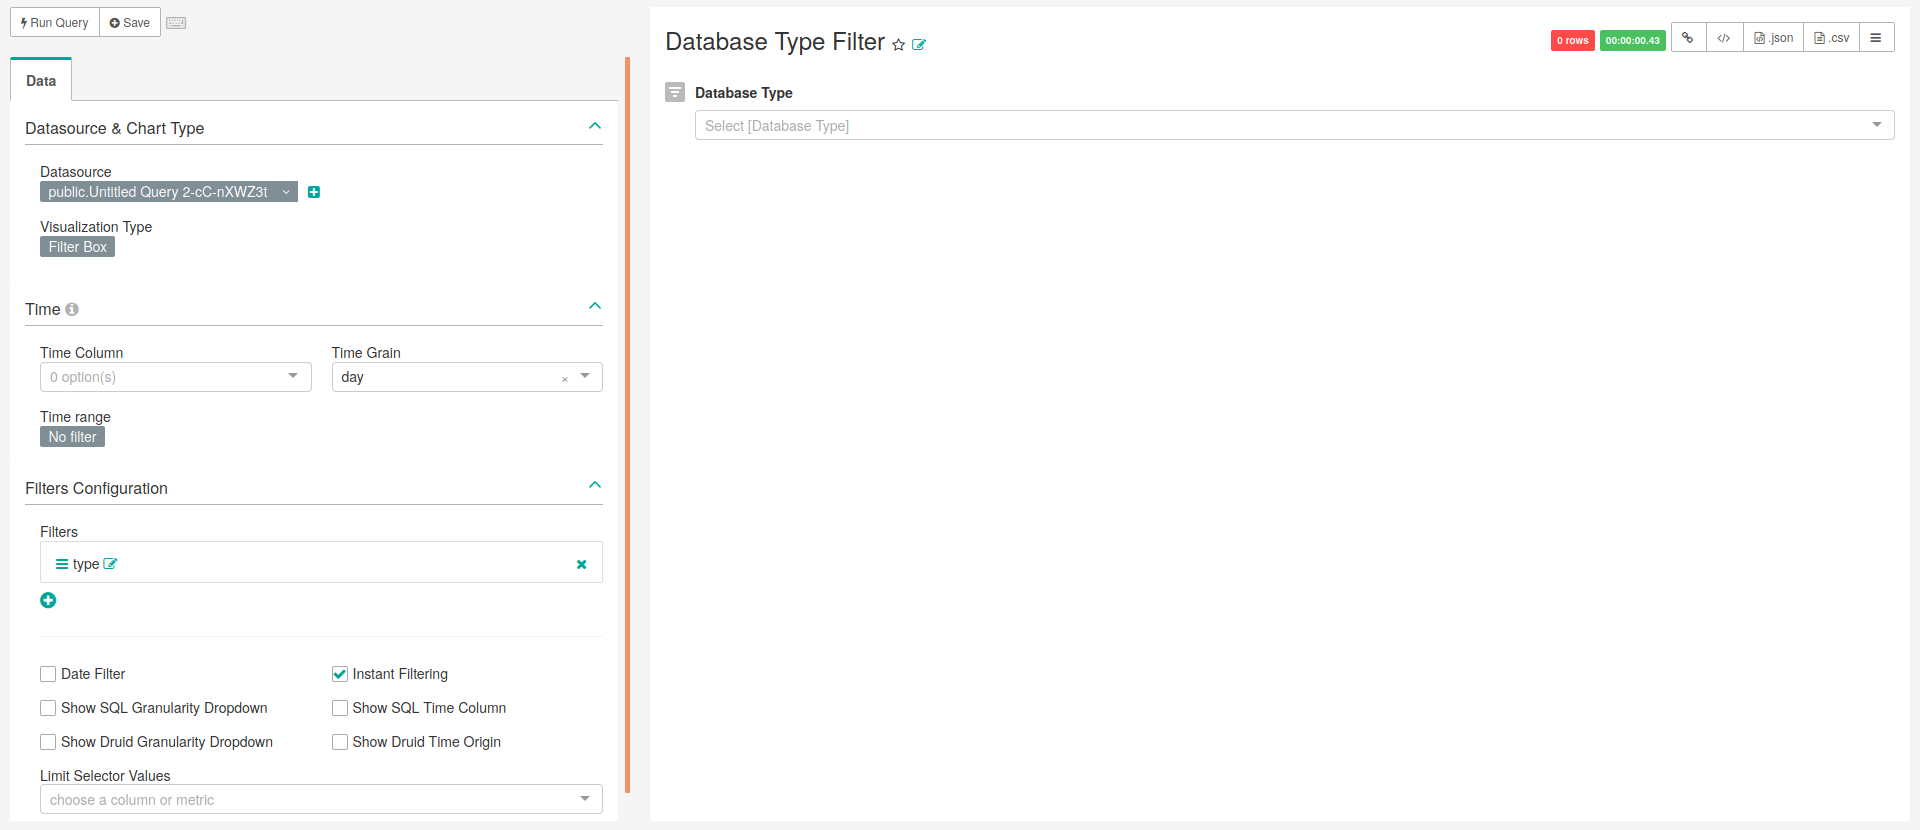
\includegraphics[width=1\linewidth]{images/databaseTypeFilter} \caption{Settings for creating the database type filter.}\label{fig:databaseTypeFilter}
\end{figure}

\section{Country Filter}\label{country-filter}

\subsection{SQL query}\label{sql-query-1}

\begin{Shaded}
\begin{Highlighting}[]
\CommentTok{--  Country and database type filters}
\KeywordTok{SELECT}\NormalTok{ source.name, }
\NormalTok{       country.country }\KeywordTok{AS}\NormalTok{ Country, }
\NormalTok{       database_type }\KeywordTok{AS} \KeywordTok{Type}\NormalTok{,}
\NormalTok{       source.slug}
\KeywordTok{FROM}\NormalTok{ public.data_source }\KeywordTok{AS} \KeywordTok{source} \KeywordTok{INNER} \KeywordTok{JOIN}\NormalTok{ public.country }
    \KeywordTok{AS}\NormalTok{ country }\KeywordTok{ON}\NormalTok{ source.country_id=country.id;}
\end{Highlighting}
\end{Shaded}

\subsection{Chart settings}\label{chart-settings-1}

TO DO

\section{General - World Map}\label{general---world-map}

\subsection{SQL query}\label{sql-query-2}

\begin{Shaded}
\begin{Highlighting}[]
\CommentTok{--    General - World Map}
\KeywordTok{SELECT}\NormalTok{  name,}
\NormalTok{        slug,}
\NormalTok{        release_date,}
\NormalTok{        database_type }\KeywordTok{AS} \KeywordTok{Type}\NormalTok{,}
\NormalTok{        latitude,}
\NormalTok{        longitude,}
        \KeywordTok{link}\NormalTok{,}
\NormalTok{        country }\KeywordTok{AS}\NormalTok{ Country,}
\NormalTok{        continent}
\KeywordTok{FROM}\NormalTok{ public.data_source }\KeywordTok{AS} \KeywordTok{source} \KeywordTok{INNER} \KeywordTok{JOIN}\NormalTok{ public.country }
    \KeywordTok{AS}\NormalTok{ country }\KeywordTok{ON}\NormalTok{ source.country_id=country.id;}
\end{Highlighting}
\end{Shaded}

\subsection{Chart settings}\label{chart-settings-2}

TO DO

\section{General - Network Growth
(Summary)}\label{general---network-growth-summary}

\subsection{SQL query}\label{sql-query-3}

\begin{Shaded}
\begin{Highlighting}[]
\CommentTok{-- 108    General - Network Growth (Summary)}
\KeywordTok{SELECT}\NormalTok{ data.source,}
\NormalTok{       data.country }\KeywordTok{AS}\NormalTok{ Country,}
\NormalTok{       data.database_type }\KeywordTok{AS} \KeywordTok{Type}\NormalTok{,}
       \CommentTok{--cast(stratum_1 as INTEGER )*30 AS Days,}
\NormalTok{       data.release_date - }\FunctionTok{cast}\NormalTok{(stratum_1 }\KeywordTok{AS} \DataTypeTok{INTEGER}\NormalTok{) * }
       \DataTypeTok{INTERVAL} \StringTok{'1 month'} \KeywordTok{as} \DataTypeTok{Time}\NormalTok{,}
\NormalTok{       count_value                   }\KeywordTok{AS} \FunctionTok{count}
\KeywordTok{FROM}\NormalTok{ (}
     \KeywordTok{SELECT}\NormalTok{ source.name              }\KeywordTok{AS} \KeywordTok{source}\NormalTok{,}
\NormalTok{            achilles.analysis_id     }\KeywordTok{AS}\NormalTok{ analysis_id,}
\NormalTok{            achilles.stratum_1,}
\NormalTok{            achilles.stratum_2,}
\NormalTok{            achilles.stratum_3,}
\NormalTok{            achilles.stratum_4,}
\NormalTok{            achilles.stratum_5,}
\NormalTok{            achilles.count_value,}
\NormalTok{            country.country,}
\NormalTok{            source.database_type, }
\NormalTok{            source.release_date}
     \KeywordTok{FROM}\NormalTok{ public.achilles_results }\KeywordTok{AS}\NormalTok{ achilles }\KeywordTok{INNER} \KeywordTok{JOIN} 
\NormalTok{        public.data_source }\KeywordTok{AS} \KeywordTok{source} \KeywordTok{ON}
\NormalTok{        achilles.data_source_id=source.id}
     \KeywordTok{INNER} \KeywordTok{JOIN}\NormalTok{ public.country }\KeywordTok{AS}\NormalTok{ country }\KeywordTok{ON} 
\NormalTok{        source.country_id=country.id}
\NormalTok{     ) }\KeywordTok{data}
\KeywordTok{WHERE}\NormalTok{ analysis_id = }\DecValTok{108}\NormalTok{;}
\end{Highlighting}
\end{Shaded}

\subsection{Chart settings}\label{chart-settings-3}

TO DO

\section{General - Network Growth by
Date}\label{general---network-growth-by-date}

\subsection{SQL query}\label{sql-query-4}

\begin{Shaded}
\begin{Highlighting}[]
\CommentTok{-- 108    General - Network Growth by Date}
\KeywordTok{SELECT}\NormalTok{ data.source,}
\NormalTok{       data.country }\KeywordTok{AS}\NormalTok{ Country,}
\NormalTok{       data.database_type }\KeywordTok{AS} \KeywordTok{Type}\NormalTok{,}
       \FunctionTok{cast}\NormalTok{(stratum_1 }\KeywordTok{as} \DataTypeTok{Integer}\NormalTok{)*}\DecValTok{30} \KeywordTok{AS} \DataTypeTok{DAY}\NormalTok{,}
\NormalTok{       count_value                   }\KeywordTok{AS} \FunctionTok{count}
\KeywordTok{FROM}\NormalTok{ (}
     \KeywordTok{SELECT}\NormalTok{ source.name              }\KeywordTok{AS} \KeywordTok{source}\NormalTok{,}
\NormalTok{            achilles.analysis_id     }\KeywordTok{AS}\NormalTok{ analysis_id,}
\NormalTok{            achilles.stratum_1,}
\NormalTok{            achilles.stratum_2,}
\NormalTok{            achilles.stratum_3,}
\NormalTok{            achilles.stratum_4,}
\NormalTok{            achilles.stratum_5,}
\NormalTok{            achilles.count_value,}
\NormalTok{            country.country,}
\NormalTok{            source.database_type}
     \KeywordTok{FROM}\NormalTok{ public.achilles_results }\KeywordTok{AS}\NormalTok{ achilles }\KeywordTok{INNER} \KeywordTok{JOIN} 
\NormalTok{        public.data_source }\KeywordTok{AS} \KeywordTok{source} \KeywordTok{ON} 
\NormalTok{        achilles.data_source_id=source.id}
     \KeywordTok{INNER} \KeywordTok{JOIN}\NormalTok{ public.country }\KeywordTok{AS}\NormalTok{ country }\KeywordTok{ON} 
\NormalTok{        source.country_id=country.id}
\NormalTok{     ) }\KeywordTok{data}
\KeywordTok{WHERE}\NormalTok{ analysis_id = }\DecValTok{108}\NormalTok{;}
\end{Highlighting}
\end{Shaded}

\subsection{Chart settings}\label{chart-settings-4}

TO DO

\section{General - Patients per
Country}\label{general---patients-per-country}

\subsection{SQL query}\label{sql-query-5}

\begin{Shaded}
\begin{Highlighting}[]
\CommentTok{-- 1    General - Patients per Country}
\KeywordTok{SELECT}\NormalTok{ source.name,}
\NormalTok{       country.country }\KeywordTok{AS}\NormalTok{ Country,}
\NormalTok{       source.database_type }\KeywordTok{AS} \KeywordTok{Type}\NormalTok{,}
\NormalTok{       count_value }\KeywordTok{AS}\NormalTok{ patient_count,}
\NormalTok{       source.slug}
\KeywordTok{FROM}\NormalTok{ public.achilles_results }\KeywordTok{AS}\NormalTok{ achilles }
    \KeywordTok{INNER} \KeywordTok{JOIN}\NormalTok{ public.data_source }\KeywordTok{AS} \KeywordTok{source} \KeywordTok{ON} 
\NormalTok{      achilles.data_source_id=source.id}
    \KeywordTok{INNER} \KeywordTok{JOIN}\NormalTok{ public.country }\KeywordTok{AS}\NormalTok{ country }\KeywordTok{ON} 
\NormalTok{      source.country_id=country.id}
\KeywordTok{WHERE}\NormalTok{ analysis_id = }\DecValTok{1}\NormalTok{;}
\end{Highlighting}
\end{Shaded}

\subsection{Chart settings}\label{chart-settings-5}

TO DO

\section{General - Database Types per
Country}\label{general---database-types-per-country}

\subsection{SQL query}\label{sql-query-6}

\begin{Shaded}
\begin{Highlighting}[]
\CommentTok{-- 1    General - Database types per Country}
\KeywordTok{SELECT}\NormalTok{ source.name, }
\NormalTok{       country.country }\KeywordTok{AS}\NormalTok{ Country, }
\NormalTok{       database_type }\KeywordTok{AS} \KeywordTok{Type}\NormalTok{,}
\NormalTok{       count_value }\KeywordTok{AS} \OtherTok{"Nr_patients"}\NormalTok{,}
\NormalTok{       source.slug}
\KeywordTok{FROM}\NormalTok{ public.achilles_results }\KeywordTok{AS}\NormalTok{ achilles }
    \KeywordTok{INNER} \KeywordTok{JOIN}\NormalTok{ public.data_source }\KeywordTok{AS} \KeywordTok{source} \KeywordTok{ON} 
\NormalTok{      achilles.data_source_id=source.id}
    \KeywordTok{INNER} \KeywordTok{JOIN}\NormalTok{ public.country }\KeywordTok{AS}\NormalTok{ country }\KeywordTok{ON} 
\NormalTok{      source.country_id=country.id}
\KeywordTok{WHERE}\NormalTok{ analysis_id = }\DecValTok{1}\NormalTok{;}
\end{Highlighting}
\end{Shaded}

\subsection{Chart settings}\label{chart-settings-6}

TO DO

\chapter{Person}\label{person}

In this dashboard is present the `'Database Type Filter'', that was
detailed in the Chapter General. Besides, it was necessary to customize
the dashboard JSON Metadata in order to obtain the colours blue and rose
in the chart representing the gender distribution. Therefore, the
following entry should be added in the settings of this dashboard:

\begin{Shaded}
\begin{Highlighting}[]
\ErrorTok{"label_colors":} \FunctionTok{\{}
    \DataTypeTok{"Male"}\FunctionTok{:} \StringTok{"#3366FF"}\FunctionTok{,} 
    \DataTypeTok{"Female"}\FunctionTok{:} \StringTok{"#FF3399"}
\FunctionTok{\}}
\end{Highlighting}
\end{Shaded}

\section{Person - Patients by age}\label{person---patients-by-age}

\subsection{SQL query}\label{sql-query-7}

\begin{Shaded}
\begin{Highlighting}[]
\CommentTok{-- 101  Person - Patients by age}
\KeywordTok{SELECT}\NormalTok{ source.name,}
       \FunctionTok{cast}\NormalTok{(stratum_1 }\KeywordTok{as} \DataTypeTok{int}\NormalTok{) }\KeywordTok{as}\NormalTok{ Age,}
\NormalTok{       count_value }\KeywordTok{as} \FunctionTok{count}\NormalTok{, }
\NormalTok{       source.slug}
\KeywordTok{FROM}\NormalTok{ public.achilles_results }\KeywordTok{AS}\NormalTok{ achilles }\KeywordTok{INNER} \KeywordTok{JOIN} 
\NormalTok{    public.data_source }\KeywordTok{AS} \KeywordTok{source} \KeywordTok{ON} 
\NormalTok{    achilles.data_source_id=source.id}
\KeywordTok{WHERE}\NormalTok{ analysis_id = }\DecValTok{101}\NormalTok{;}
\end{Highlighting}
\end{Shaded}

\subsection{Chart settings}\label{chart-settings-7}

The main characteristics of this chart are presented in Figure
\ref{fig:personPatientsByAge}, being the following:

\begin{itemize}
\tightlist
\item
  \textbf{Data Tab}:

  \begin{itemize}
  \tightlist
  \item
    \textbf{Visualization Type}: Bar Chart
  \item
    \textbf{Time range}: No filter
  \item
    \textbf{Metrics}: MAX(count)
  \item
    \textbf{Filters}: Empty
  \item
    \textbf{Series}: age
  \item
    \textbf{Breakdowns}: name
  \item
    \textbf{Row limit}: Empty
  \item
    \textbf{Contribution}: Not checked
  \end{itemize}
\item
  \textbf{Costumize Tab}:

  \begin{itemize}
  \tightlist
  \item
    \textbf{Y Axis Label}: Count
  \item
    \textbf{X Axis Label}: Age
  \item
    \textbf{Legend}: Checked
  \item
    \textbf{Stacked Bars}: Checked
  \item
    \textbf{Bar Values}: Not checked
  \item
    \textbf{Sort Bars}: Checked
  \item
    \textbf{Extra Controls}: Not checked
  \item
    \textbf{Reduce X ticks}: Checked
  \end{itemize}
\end{itemize}

\begin{figure}
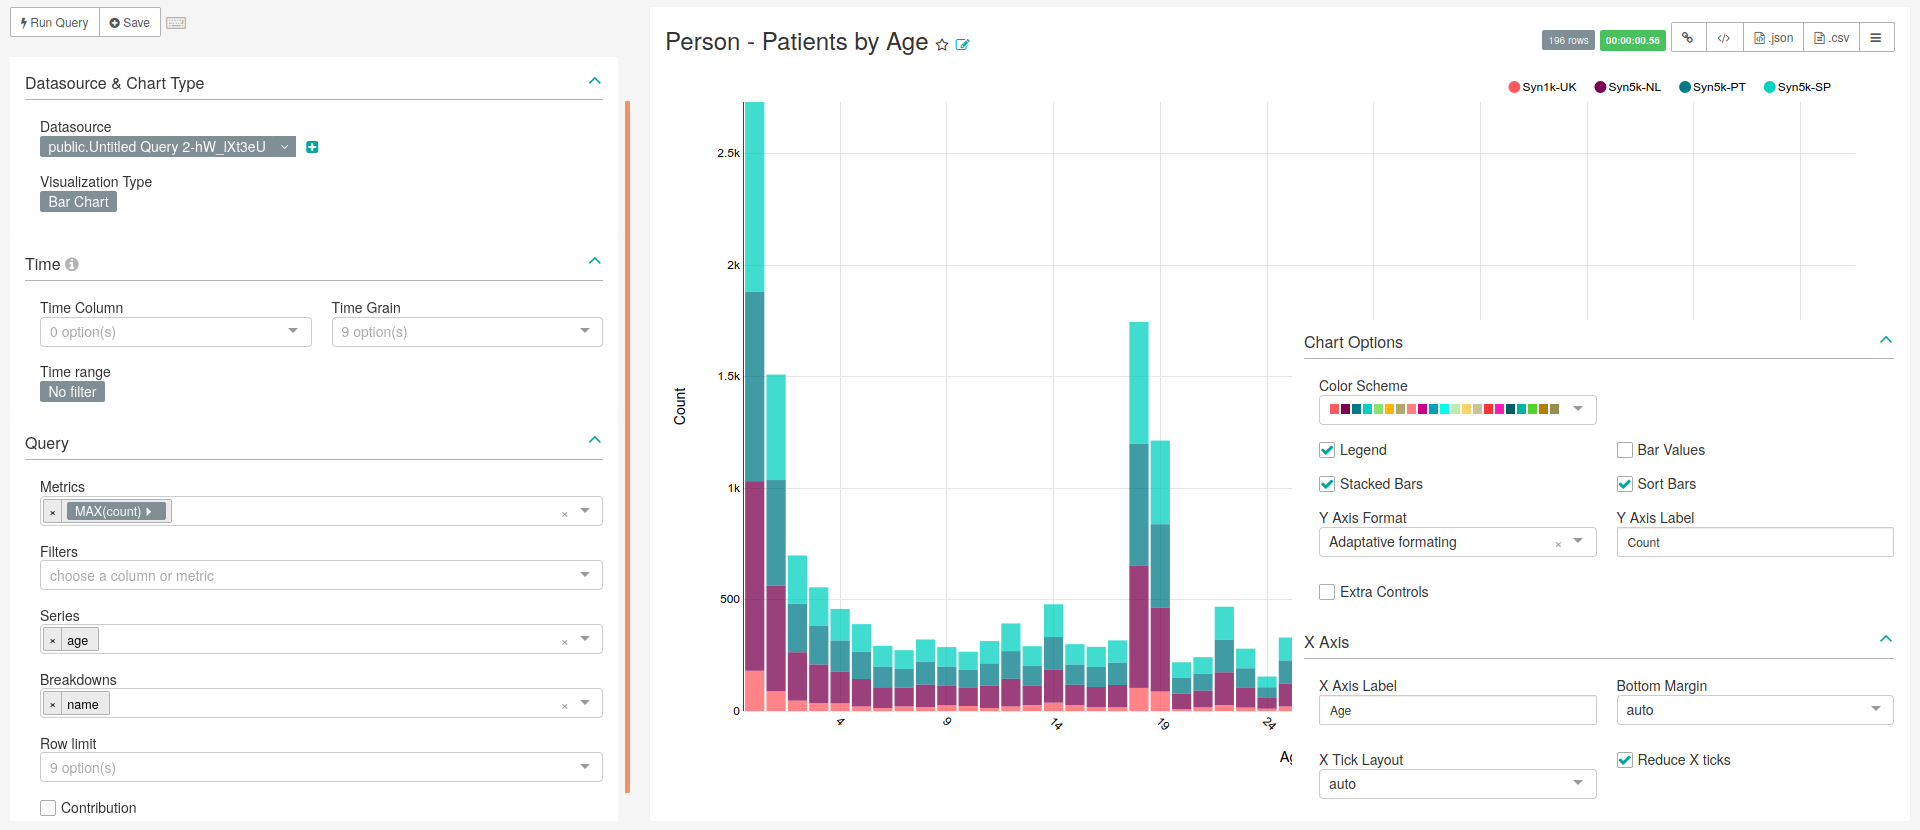
\includegraphics[width=1\linewidth]{images/personPatientsByAge} \caption{Settings for creating chart representing patient by age (bar chart). Image changed to contain information hidden in the customize menu.}\label{fig:personPatientsByAge}
\end{figure}

\section{Person - Births by Year}\label{person---births-by-year}

\subsection{SQL query}\label{sql-query-8}

\begin{Shaded}
\begin{Highlighting}[]
\CommentTok{-- 3  Person - Births by year}
\KeywordTok{SELECT}\NormalTok{ source.name,}
\NormalTok{       stratum_1 }\KeywordTok{AS} \OtherTok{"Birth_year"}\NormalTok{,}
\NormalTok{       count_value }\KeywordTok{AS} \FunctionTok{count}\NormalTok{, }
\NormalTok{       source.slug}
\KeywordTok{FROM}\NormalTok{ public.achilles_results }\KeywordTok{AS}\NormalTok{ achilles }\KeywordTok{INNER} \KeywordTok{JOIN} 
\NormalTok{      public.data_source }\KeywordTok{AS} \KeywordTok{source} \KeywordTok{ON} 
\NormalTok{    achilles.data_source_id=source.id}
\KeywordTok{WHERE}\NormalTok{ analysis_id = }\DecValTok{3}\NormalTok{;}
\end{Highlighting}
\end{Shaded}

\subsection{Chart settings}\label{chart-settings-8}

The main characteristics of this chart are presented in Figure
\ref{fig:personBirthsByYear}, being the following:

\begin{itemize}
\tightlist
\item
  \textbf{Data Tab}:

  \begin{itemize}
  \tightlist
  \item
    \textbf{Visualization Type}: Bar Chart
  \item
    \textbf{Time range}: No filter
  \item
    \textbf{Metrics}: SUM(count)
  \item
    \textbf{Filters}: Empty
  \item
    \textbf{Series}: Birth\_year
  \item
    \textbf{Breakdowns}: name
  \item
    \textbf{Row limit}: Empty
  \item
    \textbf{Contribution}: Not checked
  \end{itemize}
\item
  \textbf{Costumize Tab}:

  \begin{itemize}
  \tightlist
  \item
    \textbf{Y Axis Label}: Count
  \item
    \textbf{X Axis Label}: Age
  \item
    \textbf{Legend}: Checked
  \item
    \textbf{Stacked Bars}: Checked
  \item
    \textbf{Bar Values}: Not checked
  \item
    \textbf{Sort Bars}: Checked
  \item
    \textbf{Extra Controls}: Not checked
  \item
    \textbf{Reduce X ticks}: Checked
  \end{itemize}
\end{itemize}

\begin{figure}
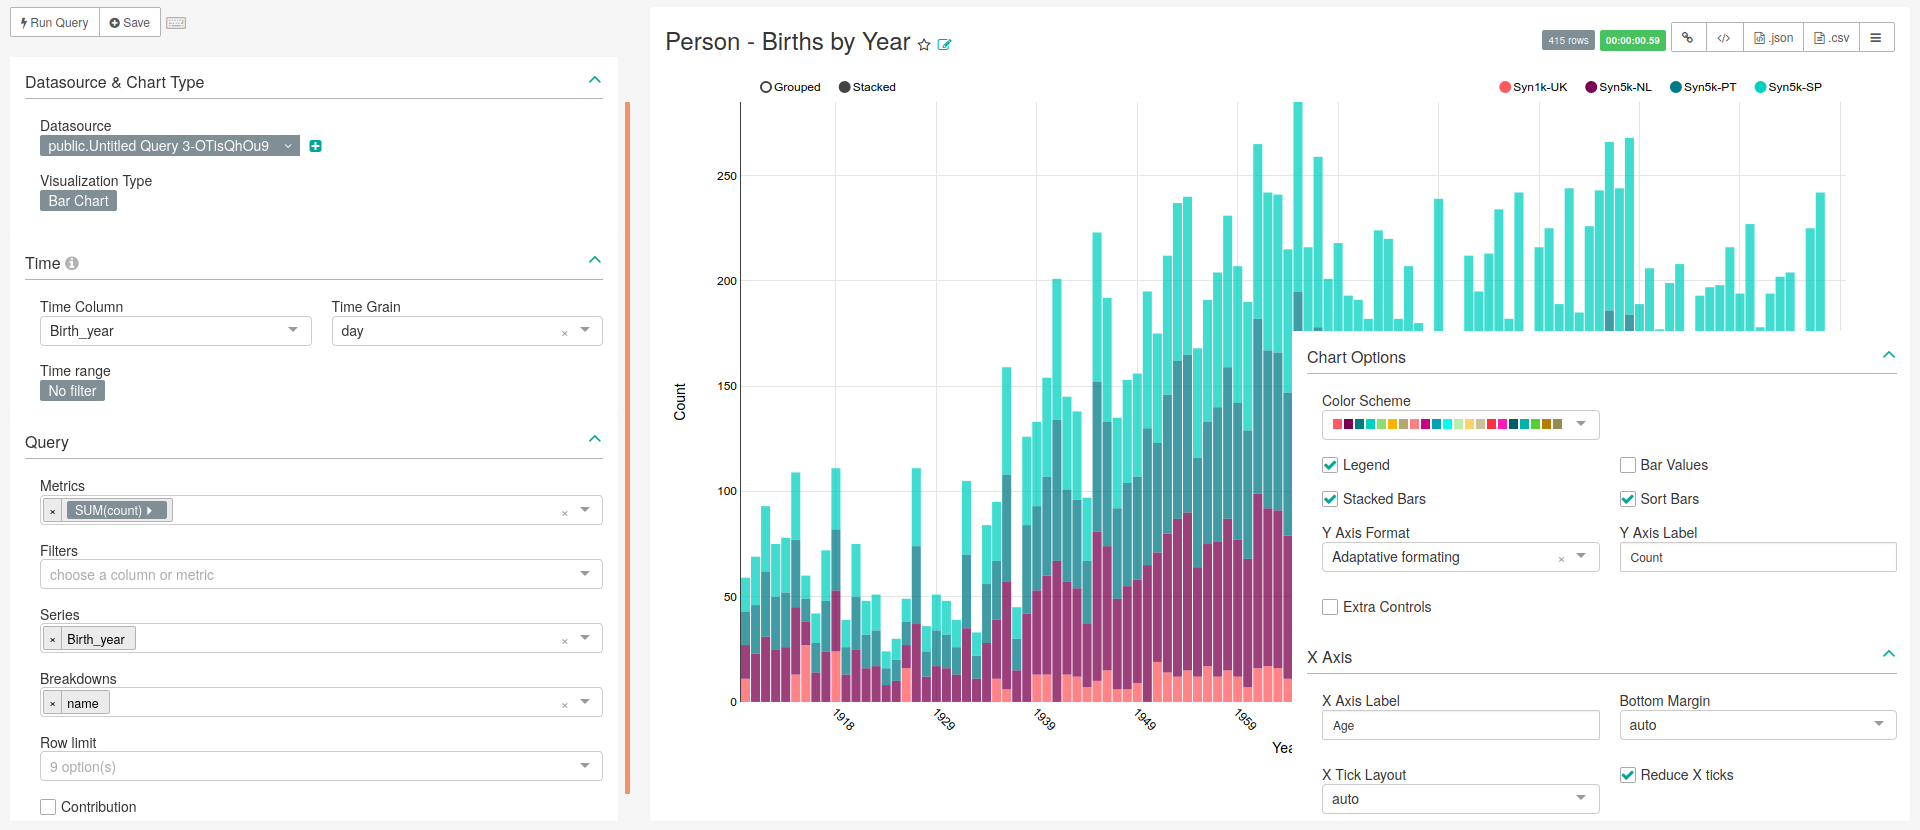
\includegraphics[width=1\linewidth]{images/personBirthsByYear} \caption{Settings for creating chart representing births by year (bar chart). Image changed to contain information hidden in the customize menu.}\label{fig:personBirthsByYear}
\end{figure}

\section{Person - Gender
Distribution}\label{person---gender-distribution}

\subsection{SQL query}\label{sql-query-9}

\begin{Shaded}
\begin{Highlighting}[]
\CommentTok{-- 2  Person - Gender distribution}
\KeywordTok{SELECT}\NormalTok{ source.name,}
\NormalTok{       concept_name }\KeywordTok{AS}\NormalTok{ Gender, }
\NormalTok{       count_value }\KeywordTok{AS}\NormalTok{ Number_of_persons,}
\NormalTok{       source.slug}
\KeywordTok{FROM}\NormalTok{ public.achilles_results }\KeywordTok{AS}\NormalTok{ achilles }\KeywordTok{INNER} \KeywordTok{JOIN} 
\NormalTok{      public.data_source }\KeywordTok{AS} \KeywordTok{source} \KeywordTok{ON} 
\NormalTok{    achilles.data_source_id = source.id}
    \KeywordTok{JOIN}\NormalTok{ (}
        \KeywordTok{SELECT} \StringTok{'8507'} \KeywordTok{AS}\NormalTok{ concept_id, }\StringTok{'Male'} \KeywordTok{AS}\NormalTok{ concept_name }\KeywordTok{UNION} 
        \KeywordTok{SELECT} \StringTok{'8532'} \KeywordTok{AS}\NormalTok{ concept_id, }\StringTok{'Female'} \KeywordTok{AS}\NormalTok{ concept_name) }\KeywordTok{AS} 
\NormalTok{        concepts }\KeywordTok{ON}\NormalTok{ achilles.stratum_1=concept_id}
\KeywordTok{WHERE}\NormalTok{ analysis_id = }\DecValTok{2}\NormalTok{;}
\end{Highlighting}
\end{Shaded}

\subsection{Chart settings}\label{chart-settings-9}

The main characteristics of this chart are presented in Figure
\ref{fig:personGenderDistribution}, being the following:

\begin{itemize}
\tightlist
\item
  \textbf{Data Tab}:

  \begin{itemize}
  \tightlist
  \item
    \textbf{Visualization Type}: Bar Chart
  \item
    \textbf{Time range}: No filter
  \item
    \textbf{Metrics}: Max(number\_of\_persons)
  \item
    \textbf{Filters}: Empty
  \item
    \textbf{Series}: name
  \item
    \textbf{Breakdowns}: gender
  \item
    \textbf{Row limit}: Empty
  \item
    \textbf{Contribution}: Checked
  \end{itemize}
\item
  \textbf{Costumize Tab}:

  \begin{itemize}
  \tightlist
  \item
    \textbf{Y Axis Label}: Empty
  \item
    \textbf{X Axis Label}: Databases
  \item
    \textbf{Legend}: Checked
  \item
    \textbf{Stacked Bars}: Checked
  \item
    \textbf{Bar Values}: Not checked
  \item
    \textbf{Sort Bars}: Checked
  \item
    \textbf{Extra Controls}: Checked
  \item
    \textbf{Reduce X ticks}: Checked
  \end{itemize}
\end{itemize}

\begin{figure}
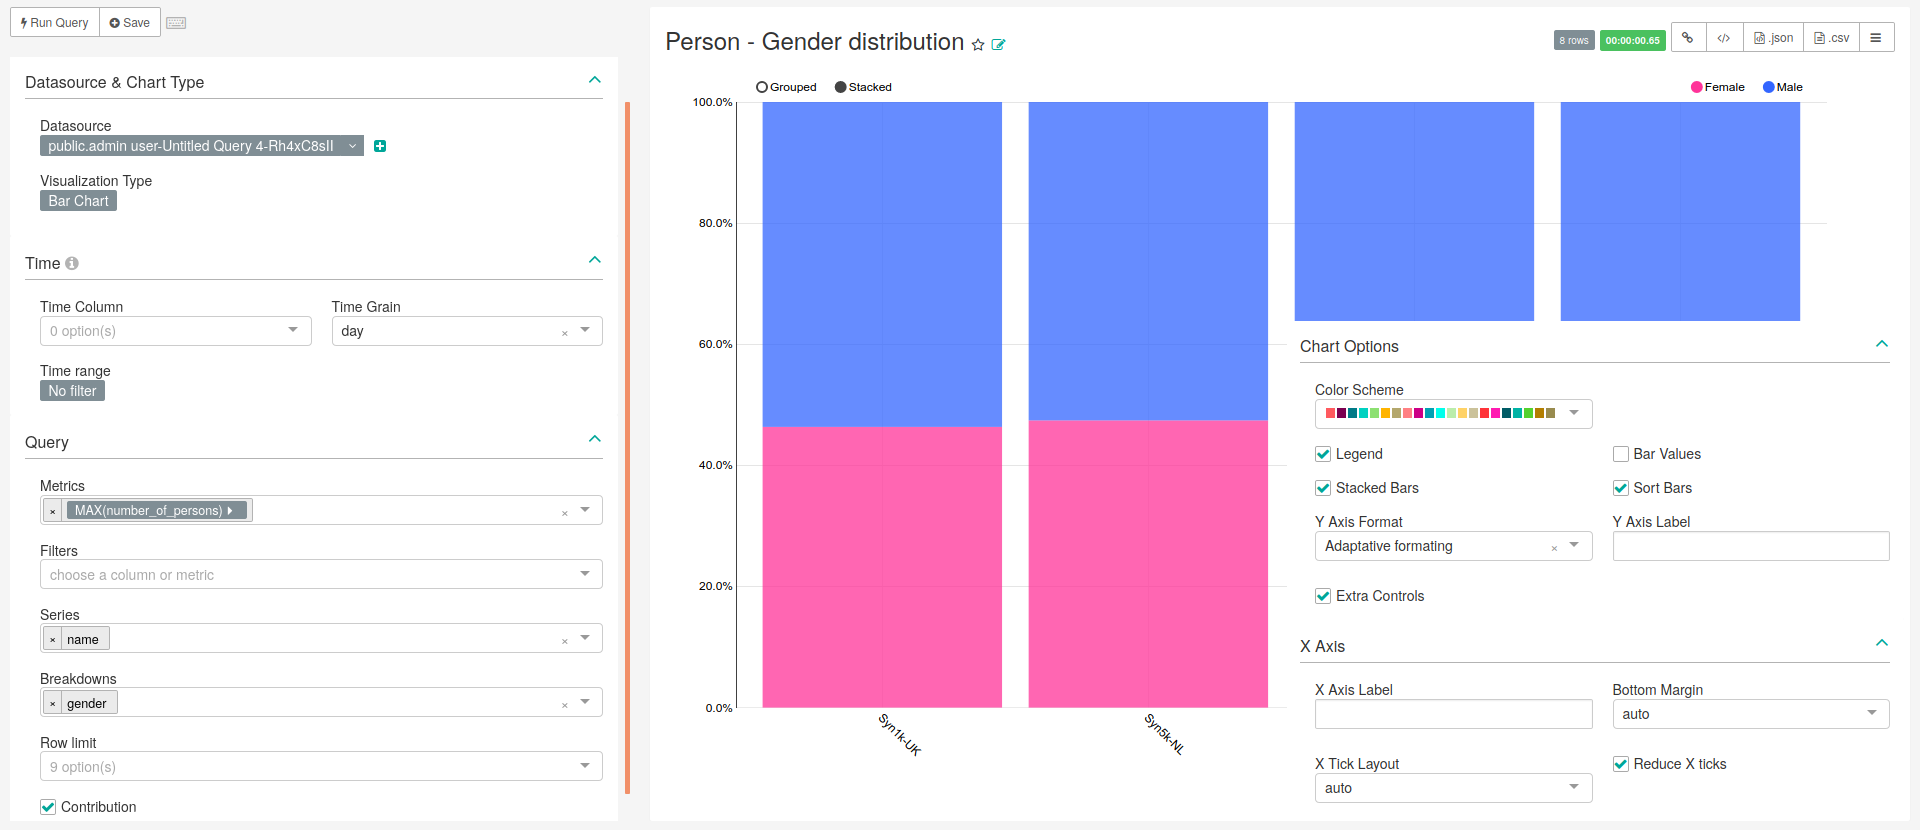
\includegraphics[width=1\linewidth]{images/personGenderDistribution} \caption{Settings for creating chart representing the gender distribution (bar chart). Image changed to contain information hidden in the customize menu.}\label{fig:personGenderDistribution}
\end{figure}

\chapter{Population Characteristics}\label{population-characteristics}

In this dashboard is present the `'Database Type Filter'', that was
detailed in the Chapter General.

\section{Population characteristics - Patients in Observation Period per
Month}\label{population-characteristics---patients-in-observation-period-per-month}

Patients in Observation Period per month (whole month)

\subsection{SQL query}\label{sql-query-10}

\begin{Shaded}
\begin{Highlighting}[]
\CommentTok{-- 110    Population characteristics - }
\CommentTok{-- Patients in Observation Period per month (whole month)}
\KeywordTok{SELECT}\NormalTok{ source.name, }
       \FunctionTok{to_date}\NormalTok{(stratum_1, }\StringTok{'YYYYMM'}\NormalTok{) }\KeywordTok{as} \DataTypeTok{Date}\NormalTok{,}
\NormalTok{       count_value }\KeywordTok{as} \OtherTok{"Nr_patients"}\NormalTok{,}
\NormalTok{       source.slug}
\KeywordTok{FROM}\NormalTok{ public.achilles_results }\KeywordTok{AS}\NormalTok{ achilles }
    \KeywordTok{INNER} \KeywordTok{JOIN}\NormalTok{ public.data_source }\KeywordTok{AS} \KeywordTok{source} \KeywordTok{ON} 
\NormalTok{      achilles.data_source_id=source.id}
\KeywordTok{WHERE}\NormalTok{ analysis_id = }\DecValTok{110}\NormalTok{;}
\end{Highlighting}
\end{Shaded}

\subsection{Chart settings}\label{chart-settings-10}

The main characteristics of this chart are presented in Figure
\ref{fig:populationCharacteristicsPatientsInObservationPeriodPerMonth},
being the following:

\begin{itemize}
\tightlist
\item
  \textbf{Data Tab}:

  \begin{itemize}
  \tightlist
  \item
    \textbf{Visualization Type}: Bar Chart
  \item
    \textbf{Time range}: No filter
  \item
    \textbf{Metrics}: MAX(Nr\_patients) as ``Num of Patients''
  \item
    \textbf{Filters}: Empty
  \item
    \textbf{Series}: date
  \item
    \textbf{Breakdowns}: name
  \item
    \textbf{Row limit}: Empty
  \item
    \textbf{Contribution}: Not checked
  \end{itemize}
\item
  \textbf{Costumize Tab}:

  \begin{itemize}
  \tightlist
  \item
    \textbf{Y Axis Label}: Number of Patients
  \item
    \textbf{X Axis Label}: Dates
  \item
    \textbf{Legend}: Checked
  \item
    \textbf{Stacked Bars}: Checked
  \item
    \textbf{Bar Values}: Not checked
  \item
    \textbf{Sort Bars}: Checked
  \item
    \textbf{Extra Controls}: Not checked
  \item
    \textbf{Reduce X ticks}: Checked
  \end{itemize}
\end{itemize}

\begin{figure}
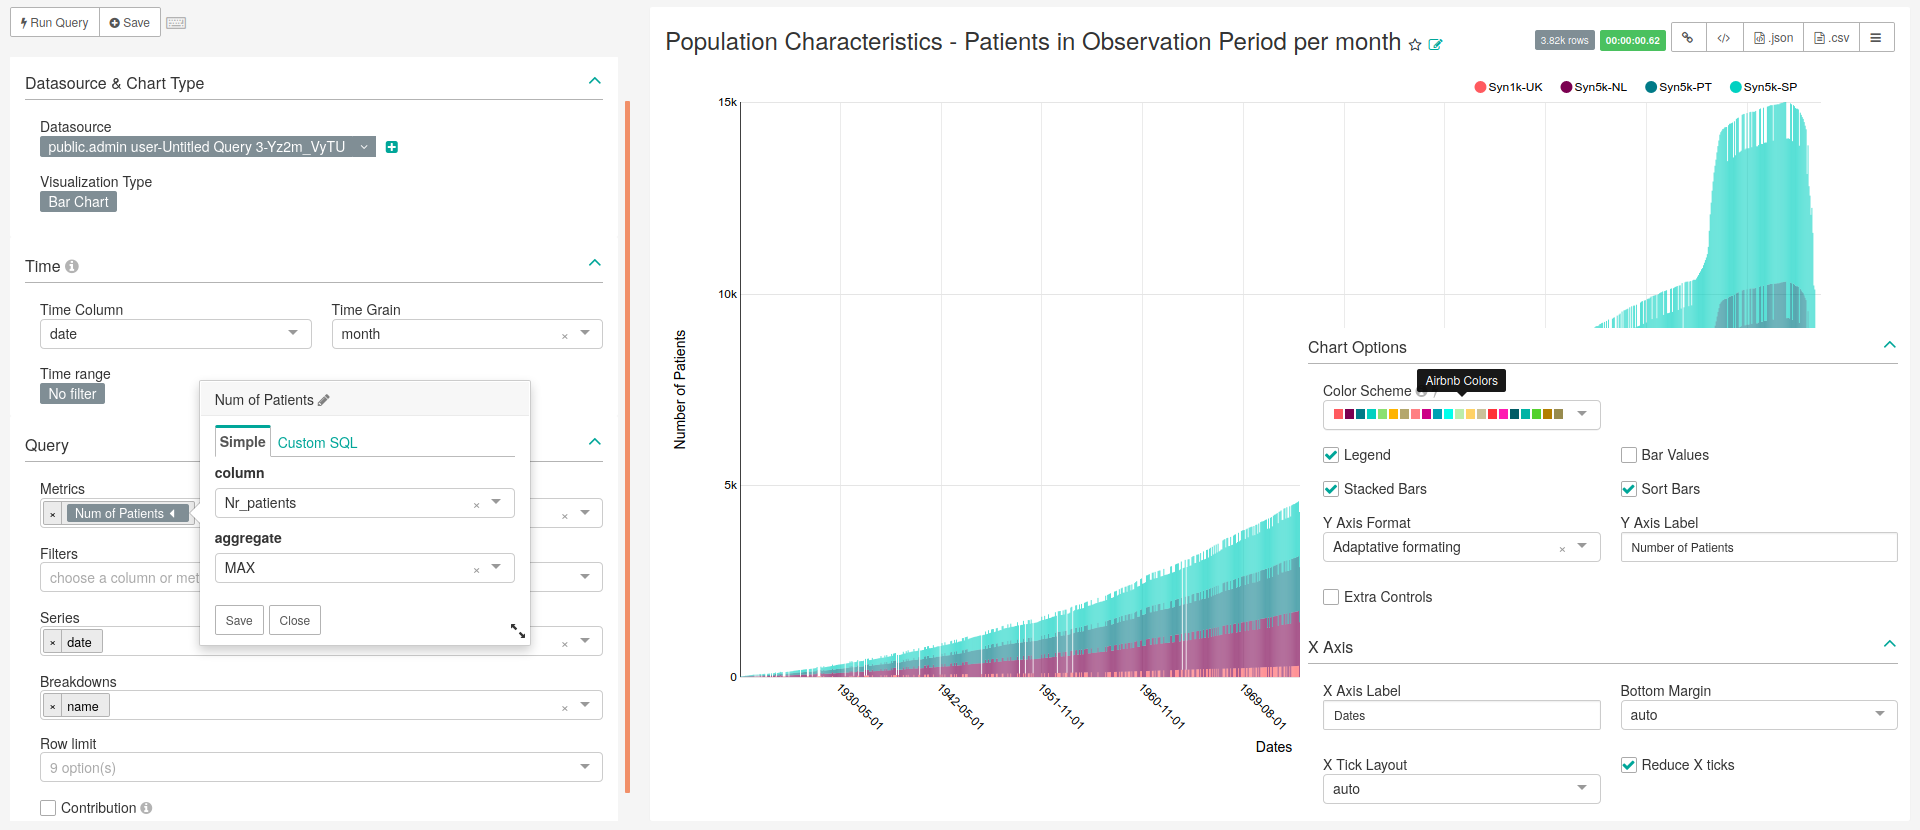
\includegraphics[width=1\linewidth]{images/populationCharacteristicsPatientsInObservationPeriodPerMonth} \caption{Settings for creating chart representing patient in observation per month (bar chart). Image changed to contain information hidden in the customize menu.}\label{fig:populationCharacteristicsPatientsInObservationPeriodPerMonth}
\end{figure}

\section{Population characteristics - Observation Period End
Dates}\label{population-characteristics---observation-period-end-dates}

\subsection{SQL query}\label{sql-query-11}

\begin{Shaded}
\begin{Highlighting}[]
\CommentTok{-- 112  Population characteristics - }
\CommentTok{--      Observation Period End Dates}
\KeywordTok{SELECT}\NormalTok{ source.name,}
       \FunctionTok{to_date}\NormalTok{(stratum_1, }\StringTok{'YYYYMM'}\NormalTok{) }\KeywordTok{as}\NormalTok{ year_month,}
\NormalTok{       count_value }\KeywordTok{as}\NormalTok{ patient_count}
\KeywordTok{FROM}\NormalTok{ public.achilles_results }\KeywordTok{AS}\NormalTok{ achilles }
    \KeywordTok{INNER} \KeywordTok{JOIN}\NormalTok{ public.data_source }\KeywordTok{AS} \KeywordTok{source} \KeywordTok{ON} 
\NormalTok{      achilles.data_source_id=source.id}
\KeywordTok{WHERE}\NormalTok{ analysis_id = }\DecValTok{112}\NormalTok{;}
\end{Highlighting}
\end{Shaded}

\subsection{Chart settings}\label{chart-settings-11}

The main characteristics of this chart are presented in Figure
\ref{fig:populationCharacteristicsObservationPeriodEndDates}, being the
following:

\begin{itemize}
\tightlist
\item
  \textbf{Data Tab}:

  \begin{itemize}
  \tightlist
  \item
    \textbf{Visualization Type}: Bar Chart
  \item
    \textbf{Time range}: No filter
  \item
    \textbf{Metrics}: SUM(patient\_count) as ``Patients''
  \item
    \textbf{Filters}: Empty
  \item
    \textbf{Series}: year\_month
  \item
    \textbf{Breakdowns}: name
  \item
    \textbf{Row limit}: Empty
  \item
    \textbf{Contribution}: Not checked
  \end{itemize}
\item
  \textbf{Costumize Tab}:

  \begin{itemize}
  \tightlist
  \item
    \textbf{Y Axis Label}: Number of Patients
  \item
    \textbf{X Axis Label}: Year
  \item
    \textbf{Legend}: Checked
  \item
    \textbf{Stacked Bars}: Checked
  \item
    \textbf{Bar Values}: Not checked
  \item
    \textbf{Sort Bars}: Checked
  \item
    \textbf{Extra Controls}: Not checked
  \item
    \textbf{Reduce X ticks}: Checked
  \end{itemize}
\end{itemize}

\begin{figure}
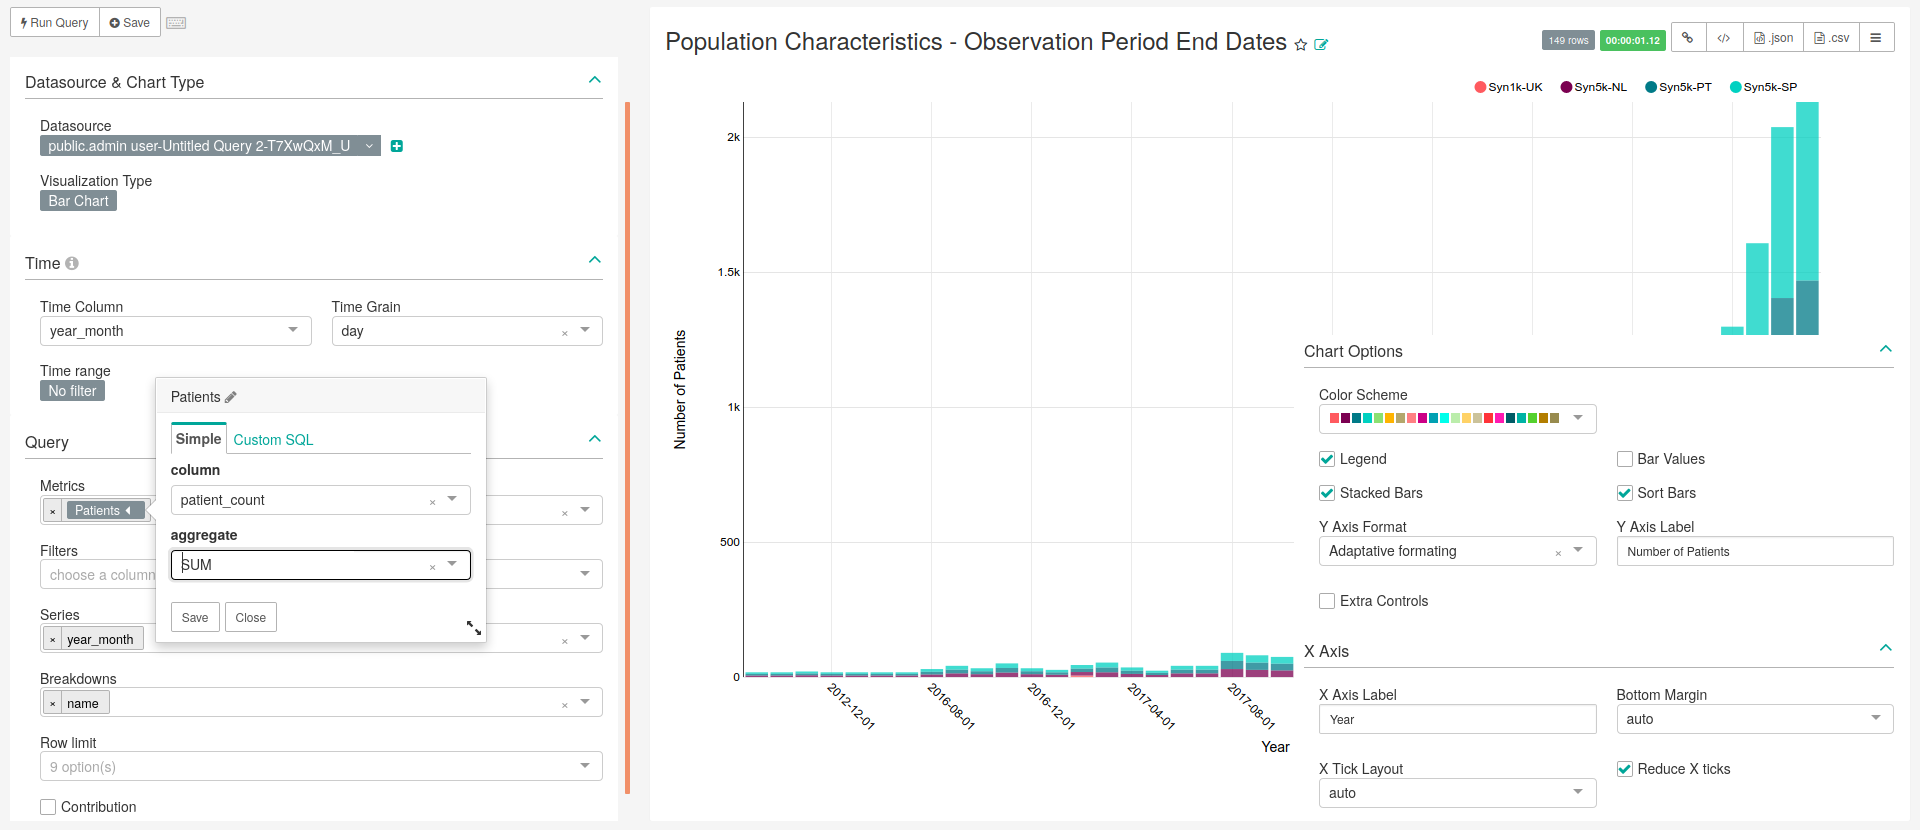
\includegraphics[width=1\linewidth]{images/populationCharacteristicsObservationPeriodEndDates} \caption{Settings for creating chart representing the number of patients at the end of their observation period (bar chart). Image changed to contain information hidden in the customize menu.}\label{fig:populationCharacteristicsObservationPeriodEndDates}
\end{figure}

\section{Population characteristics - Observation Period Start
Dates}\label{population-characteristics---observation-period-start-dates}

\subsection{SQL query}\label{sql-query-12}

\begin{Shaded}
\begin{Highlighting}[]
\CommentTok{-- 111  Population characteristics - }
\CommentTok{--      Observation Period Start Dates}
\KeywordTok{SELECT}\NormalTok{ source.name,}
       \FunctionTok{to_date}\NormalTok{(stratum_1, }\StringTok{'YYYYMM'}\NormalTok{) }\KeywordTok{as}\NormalTok{ year_month,}
\NormalTok{       count_value }\KeywordTok{as}\NormalTok{ patient_count}
\KeywordTok{FROM}\NormalTok{ public.achilles_results }\KeywordTok{AS}\NormalTok{ achilles }
    \KeywordTok{INNER} \KeywordTok{JOIN}\NormalTok{ public.data_source }\KeywordTok{AS} \KeywordTok{source} \KeywordTok{ON} 
\NormalTok{      achilles.data_source_id=source.id}
\KeywordTok{WHERE}\NormalTok{ analysis_id = }\DecValTok{111}\NormalTok{;}
\end{Highlighting}
\end{Shaded}

\subsection{Chart settings}\label{chart-settings-12}

The main characteristics of this chart are presented in Figure
\ref{fig:populationCharacteristicsObservationPeriodStartDates}, being
the following:

\begin{itemize}
\tightlist
\item
  \textbf{Data Tab}:

  \begin{itemize}
  \tightlist
  \item
    \textbf{Visualization Type}: Bar Chart
  \item
    \textbf{Time range}: No filter
  \item
    \textbf{Metrics}: SUM(patient\_count) as ``Patients''
  \item
    \textbf{Filters}: Empty
  \item
    \textbf{Series}: year\_month
  \item
    \textbf{Breakdowns}: name
  \item
    \textbf{Row limit}: Empty
  \item
    \textbf{Contribution}: Not checked
  \end{itemize}
\item
  \textbf{Costumize Tab}:

  \begin{itemize}
  \tightlist
  \item
    \textbf{Y Axis Label}: Number of Patients
  \item
    \textbf{X Axis Label}: Year
  \item
    \textbf{Legend}: Checked
  \item
    \textbf{Stacked Bars}: Checked
  \item
    \textbf{Bar Values}: Not checked
  \item
    \textbf{Sort Bars}: Checked
  \item
    \textbf{Extra Controls}: Not checked
  \item
    \textbf{Reduce X ticks}: Checked
  \end{itemize}
\end{itemize}

\begin{figure}
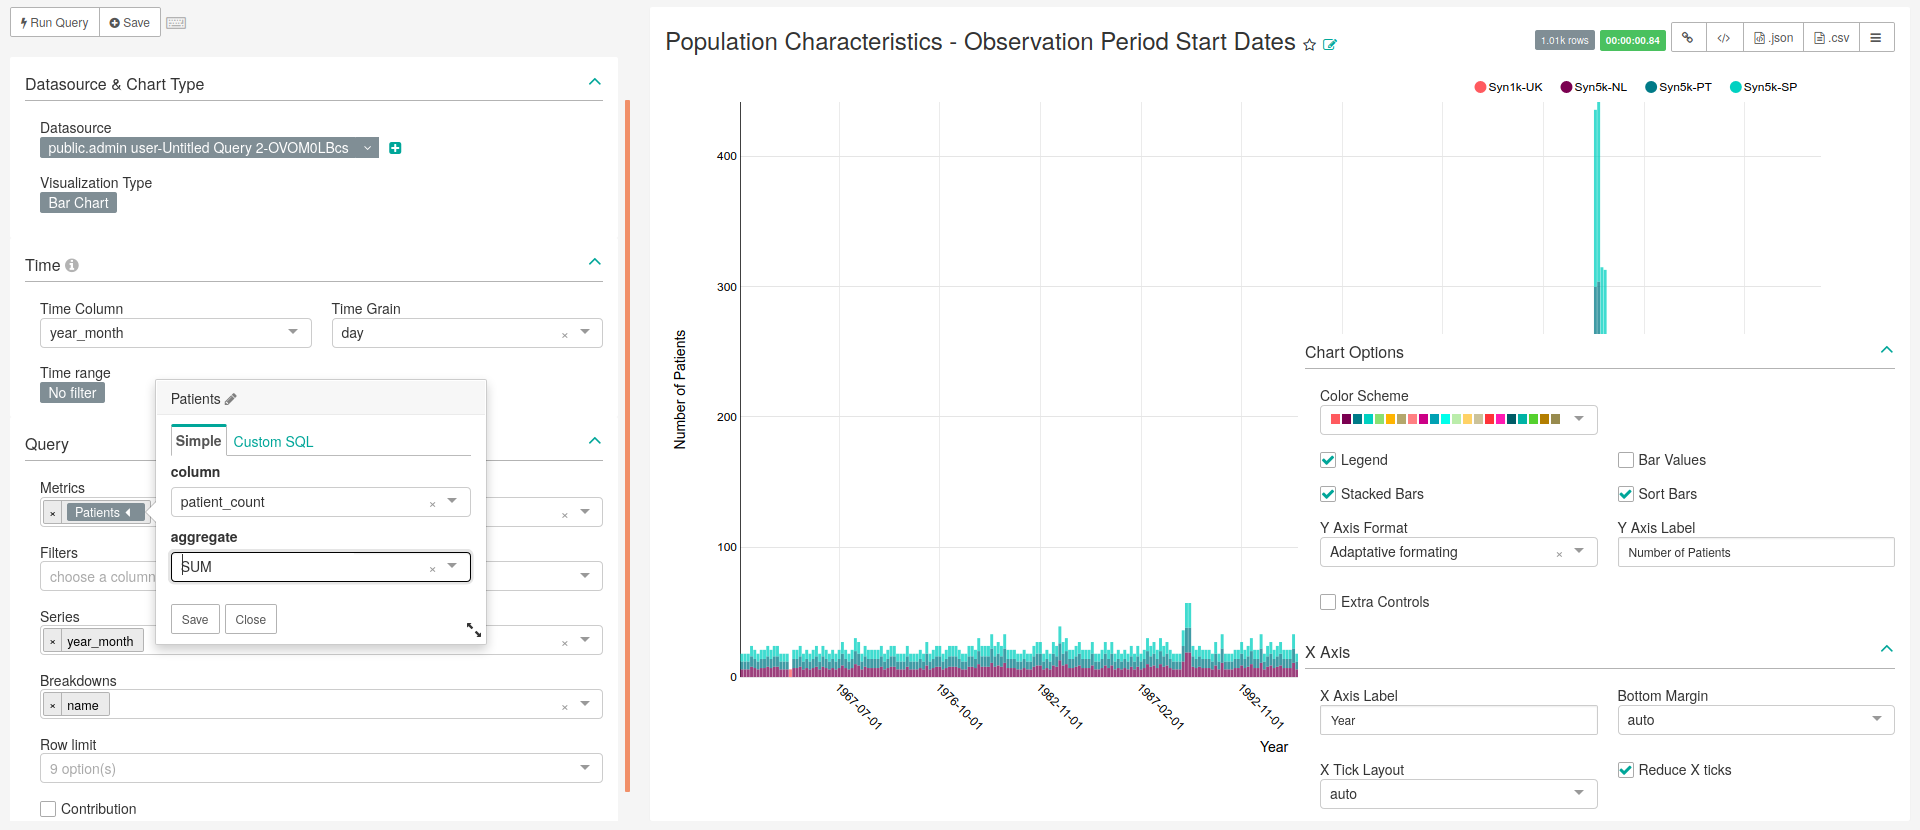
\includegraphics[width=1\linewidth]{images/populationCharacteristicsObservationPeriodStartDates} \caption{Settings for creating chart representing the number of patients at the start of their observation period (bar chart). Image changed to contain information hidden in the customize menu.}\label{fig:populationCharacteristicsObservationPeriodStartDates}
\end{figure}

\chapter{Visit}\label{visit}

In this dashboard is present the `'Database Type Filter'', that was
detailed in the Chapter General.

\section{Visit - Types}\label{visit---types}

\subsection{SQL query}\label{sql-query-13}

\begin{Shaded}
\begin{Highlighting}[]
\CommentTok{-- 201  Visit - Types}
\KeywordTok{SELECT}\NormalTok{ source.name, }
\NormalTok{       concept_name }\KeywordTok{AS} \OtherTok{"Observation"}\NormalTok{, }
\NormalTok{       count_value }\KeywordTok{AS} \OtherTok{"Nr_Observations"}\NormalTok{,}
\NormalTok{       source.slug}
\KeywordTok{FROM}\NormalTok{ public.achilles_results }\KeywordTok{AS}\NormalTok{ achilles }
    \KeywordTok{INNER} \KeywordTok{JOIN}\NormalTok{ public.data_source }\KeywordTok{AS} \KeywordTok{source} \KeywordTok{ON} 
\NormalTok{      achilles.data_source_id=source.id}
    \KeywordTok{INNER} \KeywordTok{JOIN}\NormalTok{ public.concept }\KeywordTok{ON} 
\NormalTok{      stratum_1 = }\FunctionTok{CAST}\NormalTok{(concept_id }\KeywordTok{AS}\NormalTok{ text)}
\KeywordTok{WHERE}\NormalTok{ analysis_id = }\DecValTok{201}\NormalTok{;}
\end{Highlighting}
\end{Shaded}

\subsection{Chart settings}\label{chart-settings-13}

The main characteristics of this chart are presented in Figure
\ref{fig:visitTypes}, being the following:

\begin{itemize}
\tightlist
\item
  \textbf{Data Tab}:

  \begin{itemize}
  \tightlist
  \item
    \textbf{Visualization Type}: Bar Chart
  \item
    \textbf{Time range}: No filter
  \item
    \textbf{Metrics}: MAX(Nr\_Observations) as Observations
  \item
    \textbf{Filters}: Empty
  \item
    \textbf{Series}: name
  \item
    \textbf{Breakdowns}: Observation
  \item
    \textbf{Row limit}: Empty
  \item
    \textbf{Contribution}: Not checked
  \end{itemize}
\item
  \textbf{Costumize Tab}:

  \begin{itemize}
  \tightlist
  \item
    \textbf{Y Axis Label}: Empty
  \item
    \textbf{X Axis Label}: Databases
  \item
    \textbf{Legend}: Checked
  \item
    \textbf{Stacked Bars}: Checked
  \item
    \textbf{Bar Values}: Not checked
  \item
    \textbf{Sort Bars}: Checked
  \item
    \textbf{Extra Controls}: Checked
  \item
    \textbf{Reduce X ticks}: Checked
  \end{itemize}
\end{itemize}

\begin{figure}
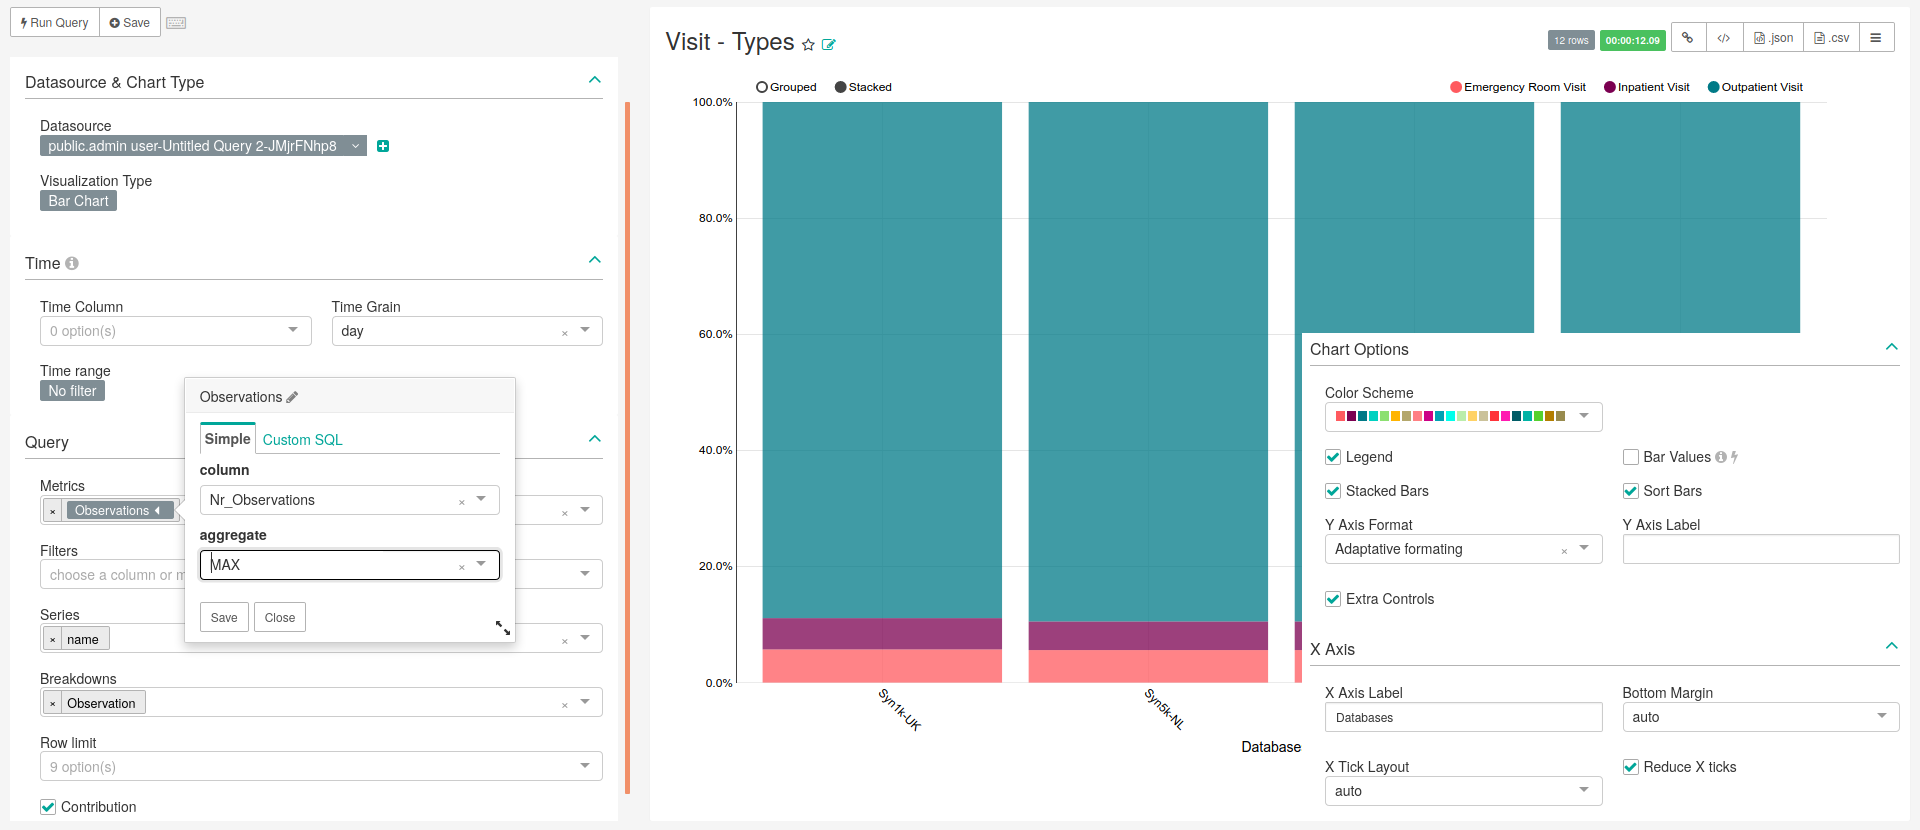
\includegraphics[width=1\linewidth]{images/visitTypes} \caption{Settings for creating chart representing the types of visit in the databases (bar chart). Image changed to contain information hidden in the customize menu.}\label{fig:visitTypes}
\end{figure}

\chapter{Death}\label{death}

In this dashboard is present the `'Database Type Filter'', that was
detailed in the Chapter General.

\section{Death - By Month per Thousand
People}\label{death---by-month-per-thousand-people}

\subsection{SQL query}\label{sql-query-14}

\begin{Shaded}
\begin{Highlighting}[]
\CommentTok{-- 502  Death - By Month per Thousand People}
\KeywordTok{SELECT}\NormalTok{ source.name,}
       \FunctionTok{to_date}\NormalTok{(stratum_1, }\StringTok{'YYYYMM'}\NormalTok{) }\KeywordTok{as} \DataTypeTok{Date}\NormalTok{,}
\NormalTok{       count_value }\KeywordTok{as} \FunctionTok{count}\NormalTok{, }
\NormalTok{       source.slug}
\KeywordTok{FROM}\NormalTok{ public.achilles_results }\KeywordTok{AS}\NormalTok{ achilles }
    \KeywordTok{INNER} \KeywordTok{JOIN}\NormalTok{ public.data_source }\KeywordTok{AS} \KeywordTok{source} \KeywordTok{ON} 
\NormalTok{      achilles.data_source_id=source.id}
\KeywordTok{WHERE}\NormalTok{ analysis_id = }\DecValTok{502}\NormalTok{;}
\end{Highlighting}
\end{Shaded}

\subsection{Chart settings}\label{chart-settings-14}

The main characteristics of this chart are presented in Figure
\ref{fig:deathByMonthPerThousandPeople}, being the following:

\begin{itemize}
\tightlist
\item
  \textbf{Data Tab}:

  \begin{itemize}
  \tightlist
  \item
    \textbf{Visualization Type}: Bar Chart
  \item
    \textbf{Time range}: No filter
  \item
    \textbf{Metrics}: MAX(count) as ``Count''
  \item
    \textbf{Filters}: Empty
  \item
    \textbf{Series}: date
  \item
    \textbf{Breakdowns}: Empty
  \item
    \textbf{Row limit}: Empty
  \item
    \textbf{Contribution}: Not checked
  \end{itemize}
\item
  \textbf{Costumize Tab}:

  \begin{itemize}
  \tightlist
  \item
    \textbf{Y Axis Label}: Number of Patients (in thousands)
  \item
    \textbf{X Axis Label}: Databases
  \item
    \textbf{Legend}: Checked
  \item
    \textbf{Stacked Bars}: Not checked
  \item
    \textbf{Bar Values}: Not checked
  \item
    \textbf{Sort Bars}: Checked
  \item
    \textbf{Extra Controls}: Not checked
  \item
    \textbf{Reduce X ticks}: Not checked
  \end{itemize}
\end{itemize}

\begin{figure}
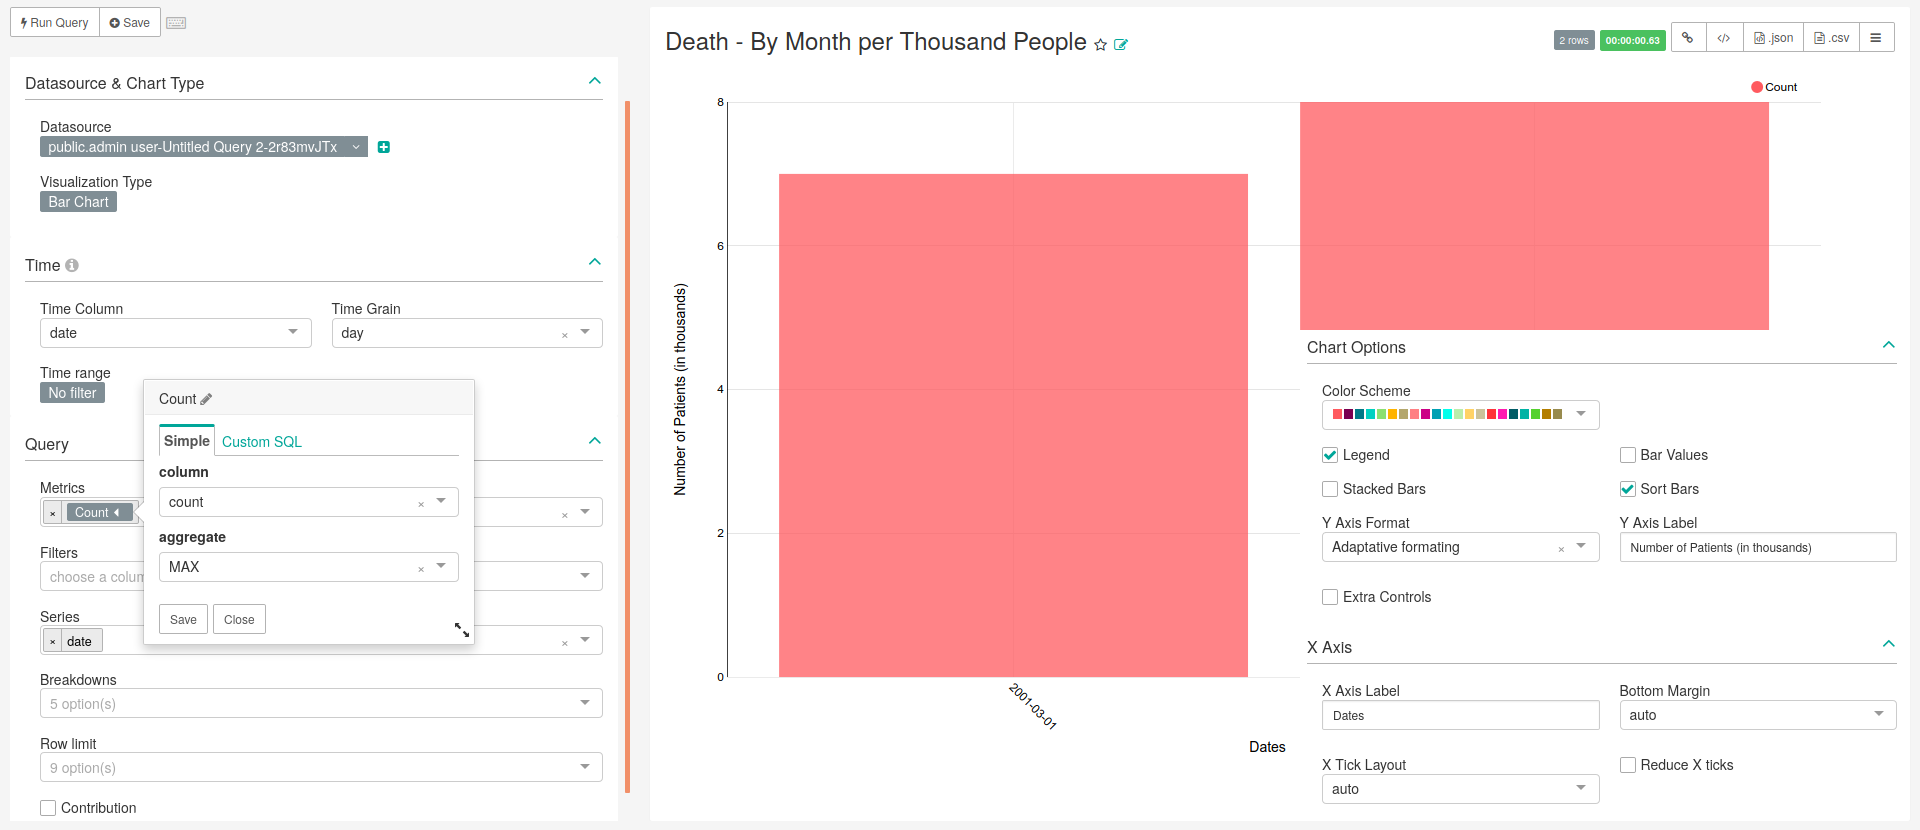
\includegraphics[width=1\linewidth]{images/deathByMonthPerThousandPeople} \caption{Settings for creating chart show in thousands the number of death patients in the network (bar chart). Image changed to contain information hidden in the customize menu.}\label{fig:deathByMonthPerThousandPeople}
\end{figure}

\section{Death - Number of Records}\label{death---number-of-records}

\subsection{SQL query}\label{sql-query-15}

\begin{Shaded}
\begin{Highlighting}[]
\CommentTok{-- 501  Death - Number of Records}
\KeywordTok{SELECT}\NormalTok{ source.name,}
\NormalTok{       count_value }\KeywordTok{as} \FunctionTok{count}\NormalTok{, }
\NormalTok{       source.slug}
\KeywordTok{FROM}\NormalTok{ public.achilles_results }\KeywordTok{AS}\NormalTok{ achilles }
    \KeywordTok{INNER} \KeywordTok{JOIN}\NormalTok{ public.data_source }\KeywordTok{AS} \KeywordTok{source} \KeywordTok{ON} 
\NormalTok{      achilles.data_source_id=source.id}
\KeywordTok{WHERE}\NormalTok{ analysis_id = }\DecValTok{501}\NormalTok{;}
\end{Highlighting}
\end{Shaded}

\subsection{Chart settings}\label{chart-settings-15}

The main characteristics of this chart are presented in Figure
\ref{fig:deathNumberOfRecords}, being the following:

\begin{itemize}
\tightlist
\item
  \textbf{Data Tab}:

  \begin{itemize}
  \tightlist
  \item
    \textbf{Visualization Type}: Bar Chart
  \item
    \textbf{Time range}: No filter
  \item
    \textbf{Metrics}: MAX(count) as ``Count''
  \item
    \textbf{Filters}: Empty
  \item
    \textbf{Series}: name
  \item
    \textbf{Breakdowns}: Empty
  \item
    \textbf{Row limit}: Empty
  \item
    \textbf{Contribution}: Not checked
  \end{itemize}
\item
  \textbf{Costumize Tab}:

  \begin{itemize}
  \tightlist
  \item
    \textbf{Y Axis Label}: Number of Patients
  \item
    \textbf{X Axis Label}: Databases
  \item
    \textbf{Legend}: Checked
  \item
    \textbf{Stacked Bars}: Not checked
  \item
    \textbf{Bar Values}: Not checked
  \item
    \textbf{Sort Bars}: Not checked
  \item
    \textbf{Extra Controls}: Not checked
  \item
    \textbf{Reduce X ticks}: Checked
  \end{itemize}
\end{itemize}

\begin{figure}
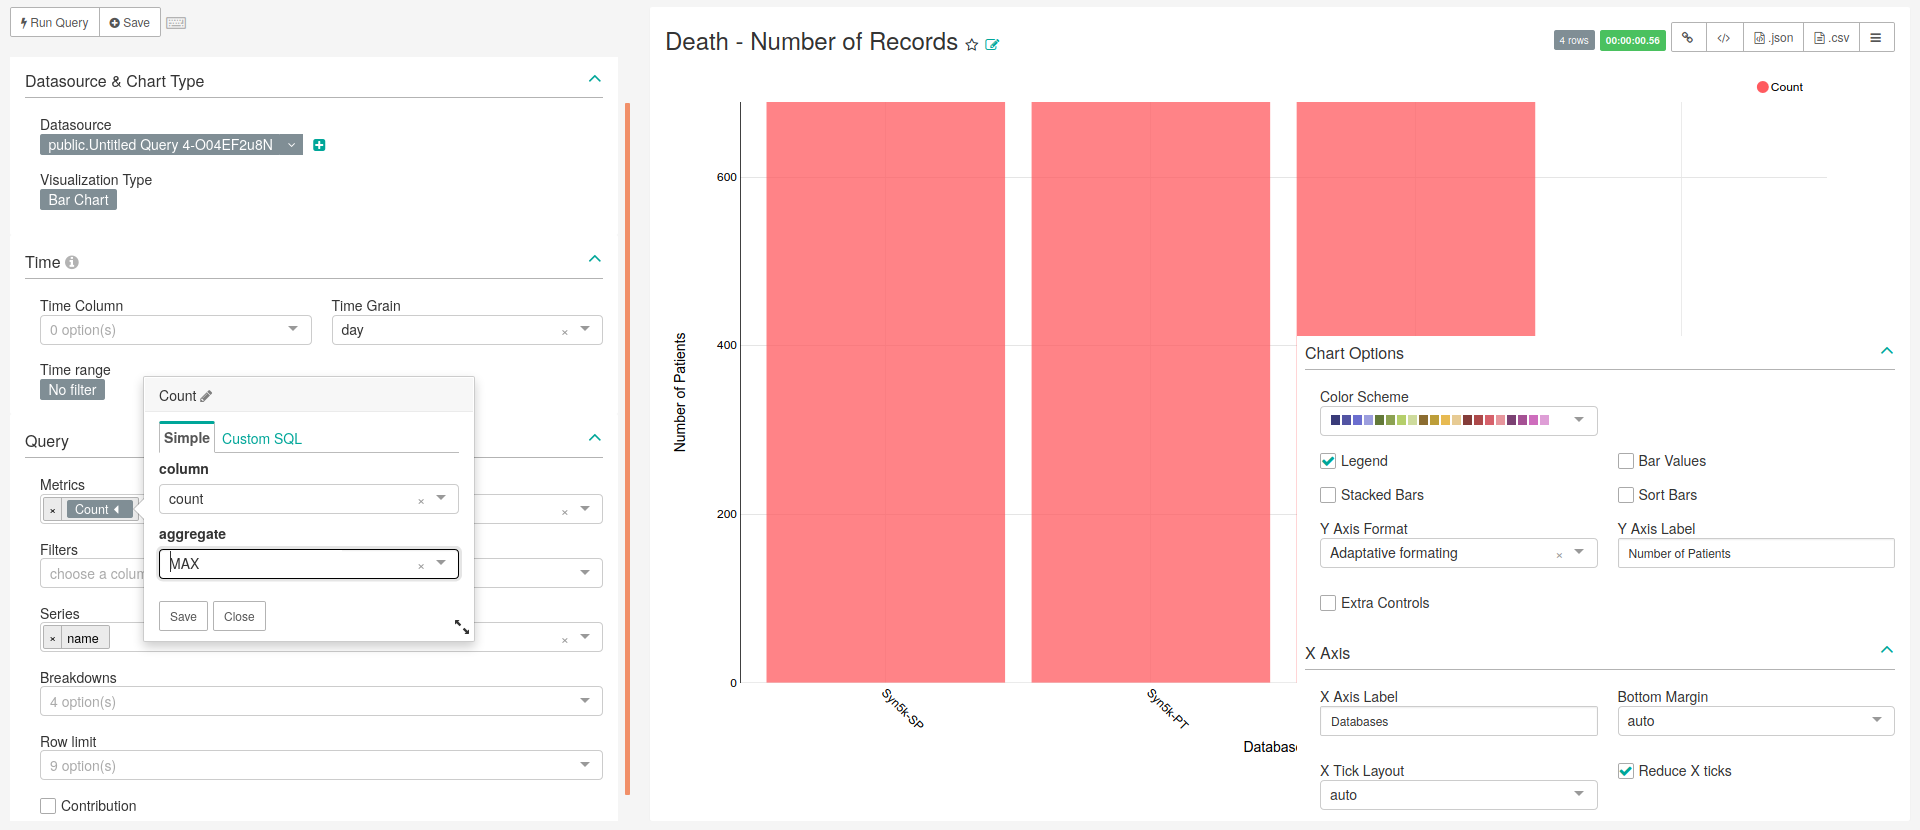
\includegraphics[width=1\linewidth]{images/deathNumberOfRecords} \caption{Settings for creating chart show the number of death patients in each database (bar chart). Image changed to contain information hidden in the customize menu.}\label{fig:deathNumberOfRecords}
\end{figure}

\chapter{Concepts}\label{concepts}

This chapter follows a different organization due to the reuse of the
same query in several charts.

\section{Concepts General Tab}\label{concepts-general-tab}

This tab uses an unique query and all the filters and charts were
created using the same output. Therefore, this dashboard is composed by
two filters, one big number, two bar charts and one table. The filters
were splitted in order to apply the filtering of one over the other one.
Figure \ref{fig:conceptsGeneralLayout} shows this dashboard's layout.

\begin{figure}
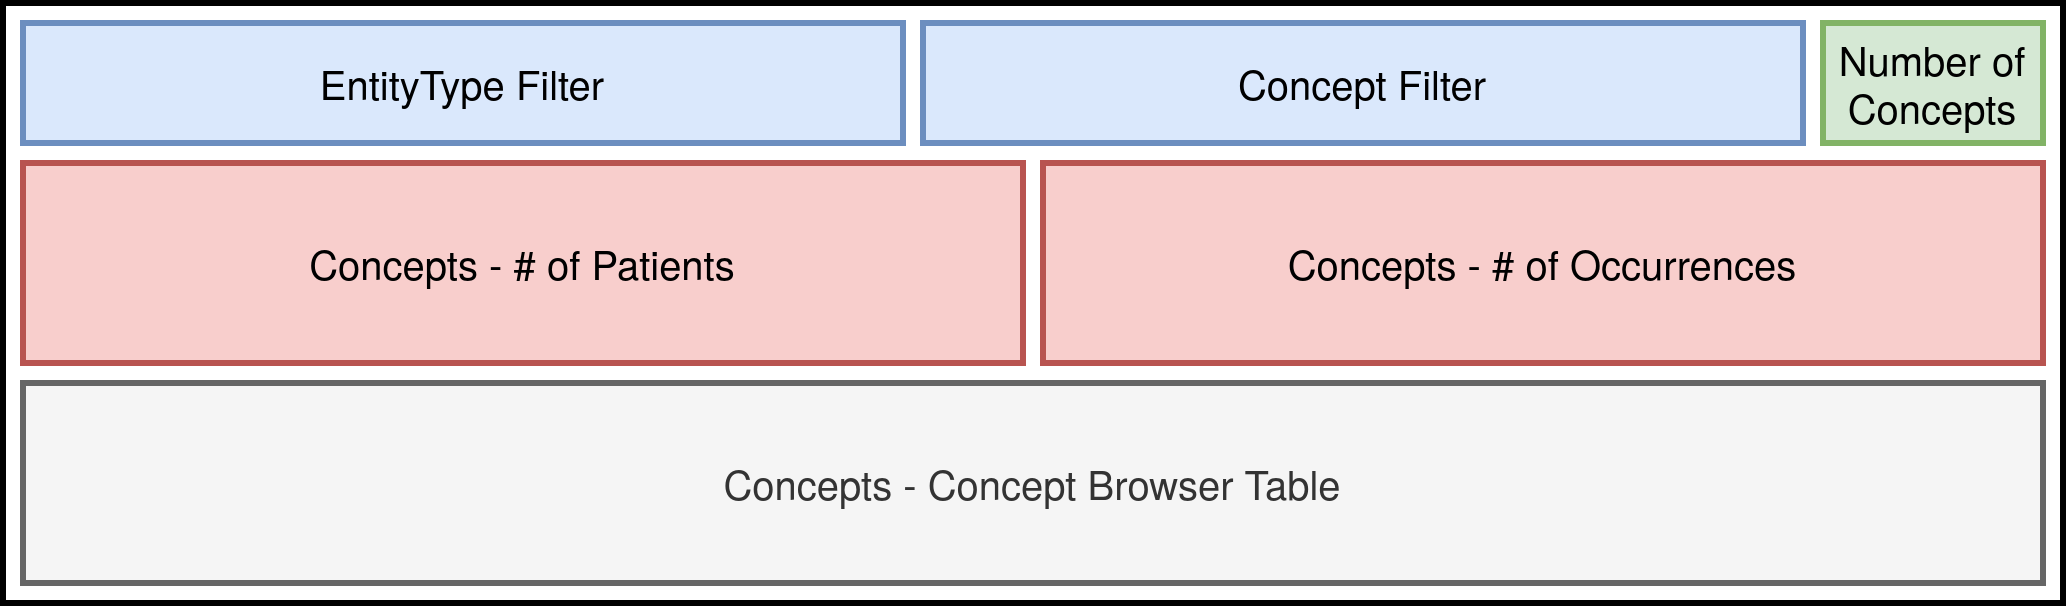
\includegraphics[width=1\linewidth]{images/conceptsGeneralLayout} \caption{Distribution of charts on the dashboard.}\label{fig:conceptsGeneralLayout}
\end{figure}

\subsection{SQL query}\label{sql-query-16}

\begin{Shaded}
\begin{Highlighting}[]
\KeywordTok{SELECT}
\NormalTok{    q1.concept_id }\KeywordTok{AS}\NormalTok{ concept_id,}
\NormalTok{    q1.concept_name }\KeywordTok{AS}\NormalTok{ concept_name,}
\NormalTok{    q1.domain_id,}
\NormalTok{    source.name,}
    \FunctionTok{sum}\NormalTok{(q1.count_value) }\KeywordTok{AS} \OtherTok{"Occurrence_count"}\NormalTok{,}
    \FunctionTok{sum}\NormalTok{(q1.count_person) }\KeywordTok{AS} \OtherTok{"Person_count"}\NormalTok{,}
    \KeywordTok{CASE} 
        \KeywordTok{WHEN} \FunctionTok{sum}\NormalTok{(q1.count_value)<=}\DecValTok{10} \KeywordTok{THEN} \StringTok{'<=10'}
        \KeywordTok{WHEN} \FunctionTok{sum}\NormalTok{(q1.count_value)<=}\DecValTok{100} \KeywordTok{THEN} \StringTok{'11-10ˆ2'}
        \KeywordTok{WHEN} \FunctionTok{sum}\NormalTok{(q1.count_value)<=}\DecValTok{1000} \KeywordTok{THEN} \StringTok{'10ˆ2-10ˆ3'}
        \KeywordTok{WHEN} \FunctionTok{sum}\NormalTok{(q1.count_value)<=}\DecValTok{10000} \KeywordTok{THEN} \StringTok{'10ˆ3-10ˆ4'}
        \KeywordTok{WHEN} \FunctionTok{sum}\NormalTok{(q1.count_value)<=}\DecValTok{100000} \KeywordTok{THEN} \StringTok{'10ˆ4-10ˆ5'}
        \KeywordTok{WHEN} \FunctionTok{sum}\NormalTok{(q1.count_value)<=}\DecValTok{1000000} \KeywordTok{THEN} \StringTok{'10ˆ5-10ˆ6'}
        \KeywordTok{ELSE} \StringTok{'>10ˆ6'}
    \KeywordTok{END} \KeywordTok{AS} \OtherTok{"magnitude_occurrences"}\NormalTok{,}
    \KeywordTok{CASE} 
        \KeywordTok{WHEN} \FunctionTok{sum}\NormalTok{(q1.count_person)<=}\DecValTok{10} \KeywordTok{THEN} \StringTok{'<=10'}
        \KeywordTok{WHEN} \FunctionTok{sum}\NormalTok{(q1.count_person)<=}\DecValTok{100} \KeywordTok{THEN} \StringTok{'11-10ˆ2'}
        \KeywordTok{WHEN} \FunctionTok{sum}\NormalTok{(q1.count_person)<=}\DecValTok{1000} \KeywordTok{THEN} \StringTok{'10ˆ2-10ˆ3'}
        \KeywordTok{WHEN} \FunctionTok{sum}\NormalTok{(q1.count_person)<=}\DecValTok{10000} \KeywordTok{THEN} \StringTok{'10ˆ3-10ˆ4'}
        \KeywordTok{WHEN} \FunctionTok{sum}\NormalTok{(q1.count_person)<=}\DecValTok{100000} \KeywordTok{THEN} \StringTok{'10ˆ4-10ˆ5'}
        \KeywordTok{WHEN} \FunctionTok{sum}\NormalTok{(q1.count_person)<=}\DecValTok{1000000} \KeywordTok{THEN} \StringTok{'10ˆ5-10ˆ6'}
        \KeywordTok{ELSE} \StringTok{'>10ˆ6'}
    \KeywordTok{END} \KeywordTok{AS} \OtherTok{"magnitude_persons"}
\KeywordTok{FROM}\NormalTok{ (}\KeywordTok{SELECT}\NormalTok{ analysis_id,}
\NormalTok{             stratum_1 concept_id,}
\NormalTok{             data_source_id,}
\NormalTok{             concept_name,}
\NormalTok{             domain_id,}
\NormalTok{             count_value, }\DecValTok{0} \KeywordTok{AS}\NormalTok{ count_person}
    \KeywordTok{FROM}\NormalTok{ achilles_results}
    \KeywordTok{JOIN}\NormalTok{ concept }\KeywordTok{ON} \FunctionTok{cast}\NormalTok{(stratum_1 }\KeywordTok{AS}\NormalTok{ BIGINT)=concept_id}
    \KeywordTok{WHERE}\NormalTok{ analysis_id }\KeywordTok{in}\NormalTok{ (}\DecValTok{201}\NormalTok{, }\DecValTok{301}\NormalTok{, }\DecValTok{401}\NormalTok{, }\DecValTok{601}\NormalTok{, }\DecValTok{701}\NormalTok{, }\DecValTok{801}\NormalTok{, }\DecValTok{901}\NormalTok{, }\DecValTok{1001}\NormalTok{, }
        \DecValTok{1801}\NormalTok{)}
    \KeywordTok{UNION}\NormalTok{ (}\KeywordTok{SELECT}\NormalTok{  analysis_id,}
\NormalTok{                   stratum_1 concept_id,}
\NormalTok{                   data_source_id,}
\NormalTok{                   concept_name,}
\NormalTok{                   domain_id,}
                   \DecValTok{0} \KeywordTok{AS}\NormalTok{ count_value,}
                   \FunctionTok{sum}\NormalTok{(count_value) }\KeywordTok{AS}\NormalTok{ count_person}
            \KeywordTok{FROM}\NormalTok{  achilles_results}
            \KeywordTok{JOIN}\NormalTok{ concept }\KeywordTok{on} \FunctionTok{cast}\NormalTok{(stratum_1 }\KeywordTok{AS}\NormalTok{ BIGINT)=concept_id}
            \KeywordTok{WHERE}\NormalTok{ analysis_id }\KeywordTok{in}\NormalTok{ (}\DecValTok{202}\NormalTok{, }\DecValTok{401}\NormalTok{, }\DecValTok{601}\NormalTok{, }\DecValTok{701}\NormalTok{, }\DecValTok{801}\NormalTok{, }\DecValTok{901}\NormalTok{, }
                \DecValTok{1001}\NormalTok{, }\DecValTok{1801}\NormalTok{)}
            \KeywordTok{GROUP} \KeywordTok{BY}\NormalTok{ analysis_id, stratum_1, data_source_id, }
\NormalTok{                concept_name, domain_id) ) }\KeywordTok{AS}\NormalTok{ q1}
    \KeywordTok{INNER} \KeywordTok{JOIN}\NormalTok{ public.data_source }\KeywordTok{AS} \KeywordTok{source} \KeywordTok{ON} 
\NormalTok{        q1.data_source_id=source.id}
\KeywordTok{GROUP} \KeywordTok{BY}\NormalTok{ q1.concept_id, q1.concept_name, q1.domain_id,source.name;}
\end{Highlighting}
\end{Shaded}

\subsection{Charts}\label{charts}

\subsubsection{Entity Type Filter}\label{entity-type-filter}

This filter, which is a type of chart in Superset, was designed to be
used in the dashboard aiming the filtering of the data based on the
field `'domain\_id'`from the table'`concept''. The main characteristics
of this filter are presented in Figure \ref{fig:entityTypeFilter}, being
the following:

\begin{itemize}
\tightlist
\item
  \textbf{Data Tab}:

  \begin{itemize}
  \tightlist
  \item
    \textbf{Visualization Type}: Filter Box
  \item
    \textbf{Time range}: No filter
  \item
    \textbf{Metrics}:
  \item
    \textbf{Filters - Column}: domain\_id
  \item
    \textbf{Filters - Label}: Entity Type
  \item
    \textbf{Data Filter}: Not checked
  \item
    \textbf{Row limit}: Empty
  \item
    \textbf{Contribution}: Not checked
  \item
    \textbf{Instant Filtering}: Checked
  \item
    \textbf{Show SQL Granularity Dropdown}: Not checked
  \item
    \textbf{Show Druid Granularity Dropdown}: Not checked
  \item
    \textbf{Show SQL Time Column}: Not checked
  \item
    \textbf{Show Druid Time Origin}: Not checked
  \item
    \textbf{Limit Selector Values}: Empty
  \end{itemize}
\end{itemize}

\begin{figure}
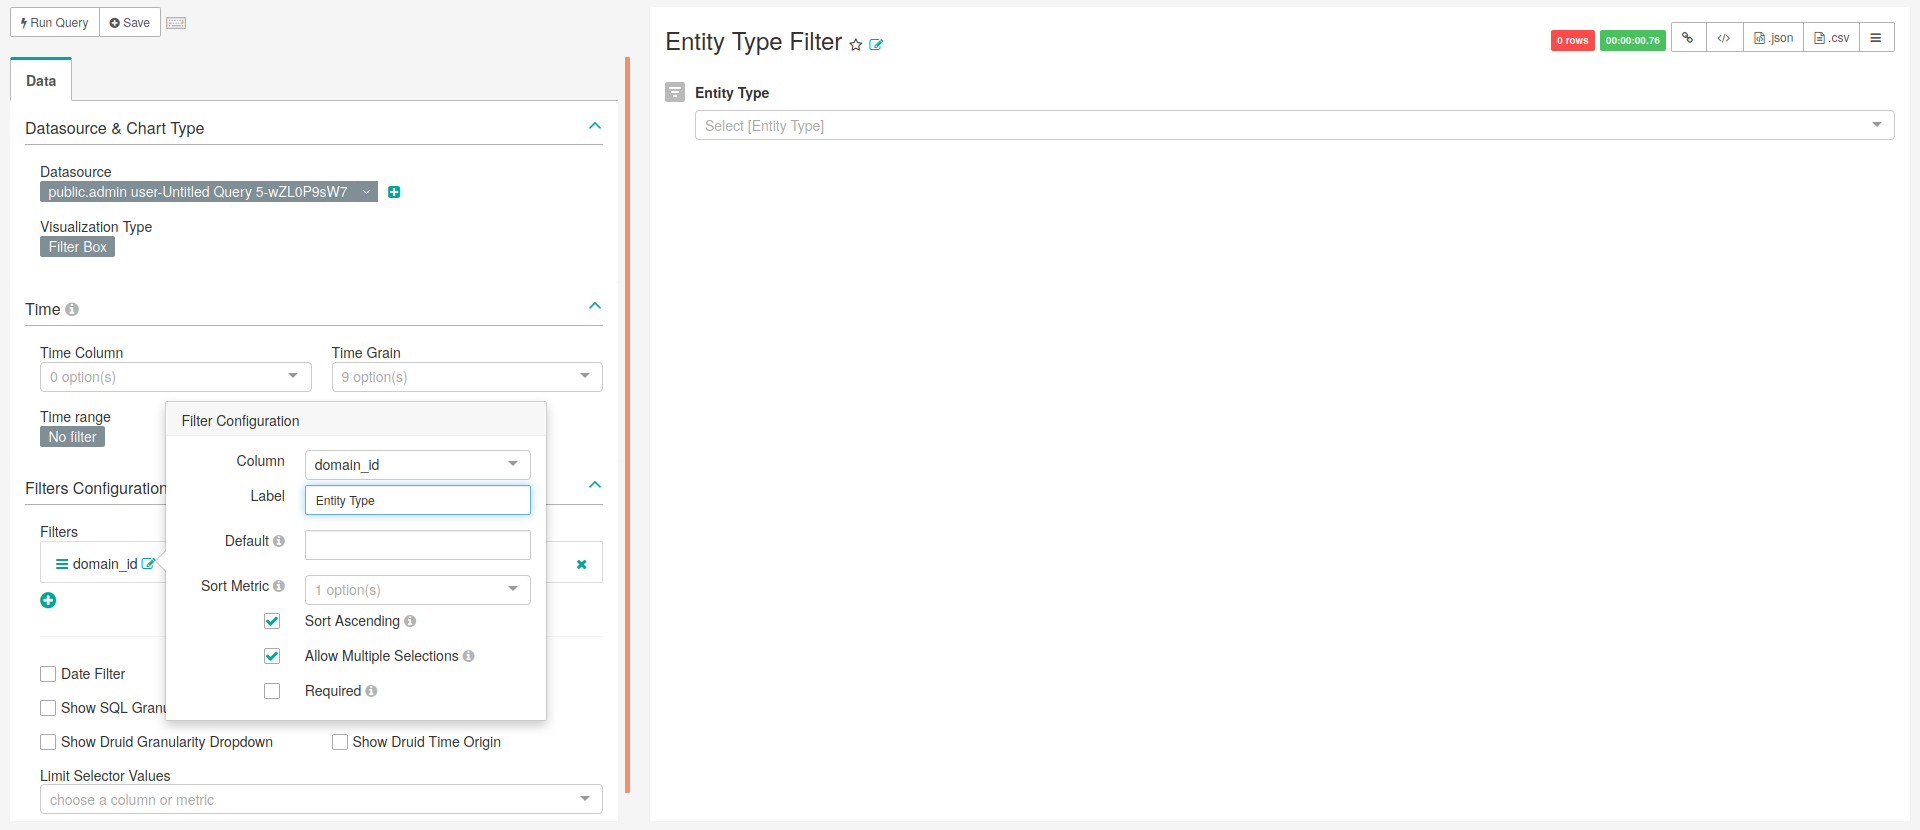
\includegraphics[width=1\linewidth]{images/entityTypeFilter} \caption{Settings for creating the database entity type filter.}\label{fig:entityTypeFilter}
\end{figure}

\subsubsection{Concept Filter}\label{concept-filter}

Similar to the previous filter, this was designed to be used in the
dashboard aiming the filtering of the data based on the field
`'concept\_name'`from the table'`concept''. The main characteristics of
this filter are presented in Figure \ref{fig:conceptFilter}, being the
following:

\begin{itemize}
\tightlist
\item
  \textbf{Data Tab}:

  \begin{itemize}
  \tightlist
  \item
    \textbf{Visualization Type}: Filter Box
  \item
    \textbf{Time range}: No filter
  \item
    \textbf{Metrics}:
  \item
    \textbf{Filters - Column}: concept\_name
  \item
    \textbf{Filters - Label}: Concept
  \item
    \textbf{Data Filter}: Not checked
  \item
    \textbf{Row limit}: Empty
  \item
    \textbf{Contribution}: Not checked
  \item
    \textbf{Instant Filtering}: Checked
  \item
    \textbf{Show SQL Granularity Dropdown}: Not checked
  \item
    \textbf{Show Druid Granularity Dropdown}: Not checked
  \item
    \textbf{Show SQL Time Column}: Not checked
  \item
    \textbf{Show Druid Time Origin}: Not checked
  \item
    \textbf{Limit Selector Values}: Empty
  \end{itemize}
\end{itemize}

\begin{figure}
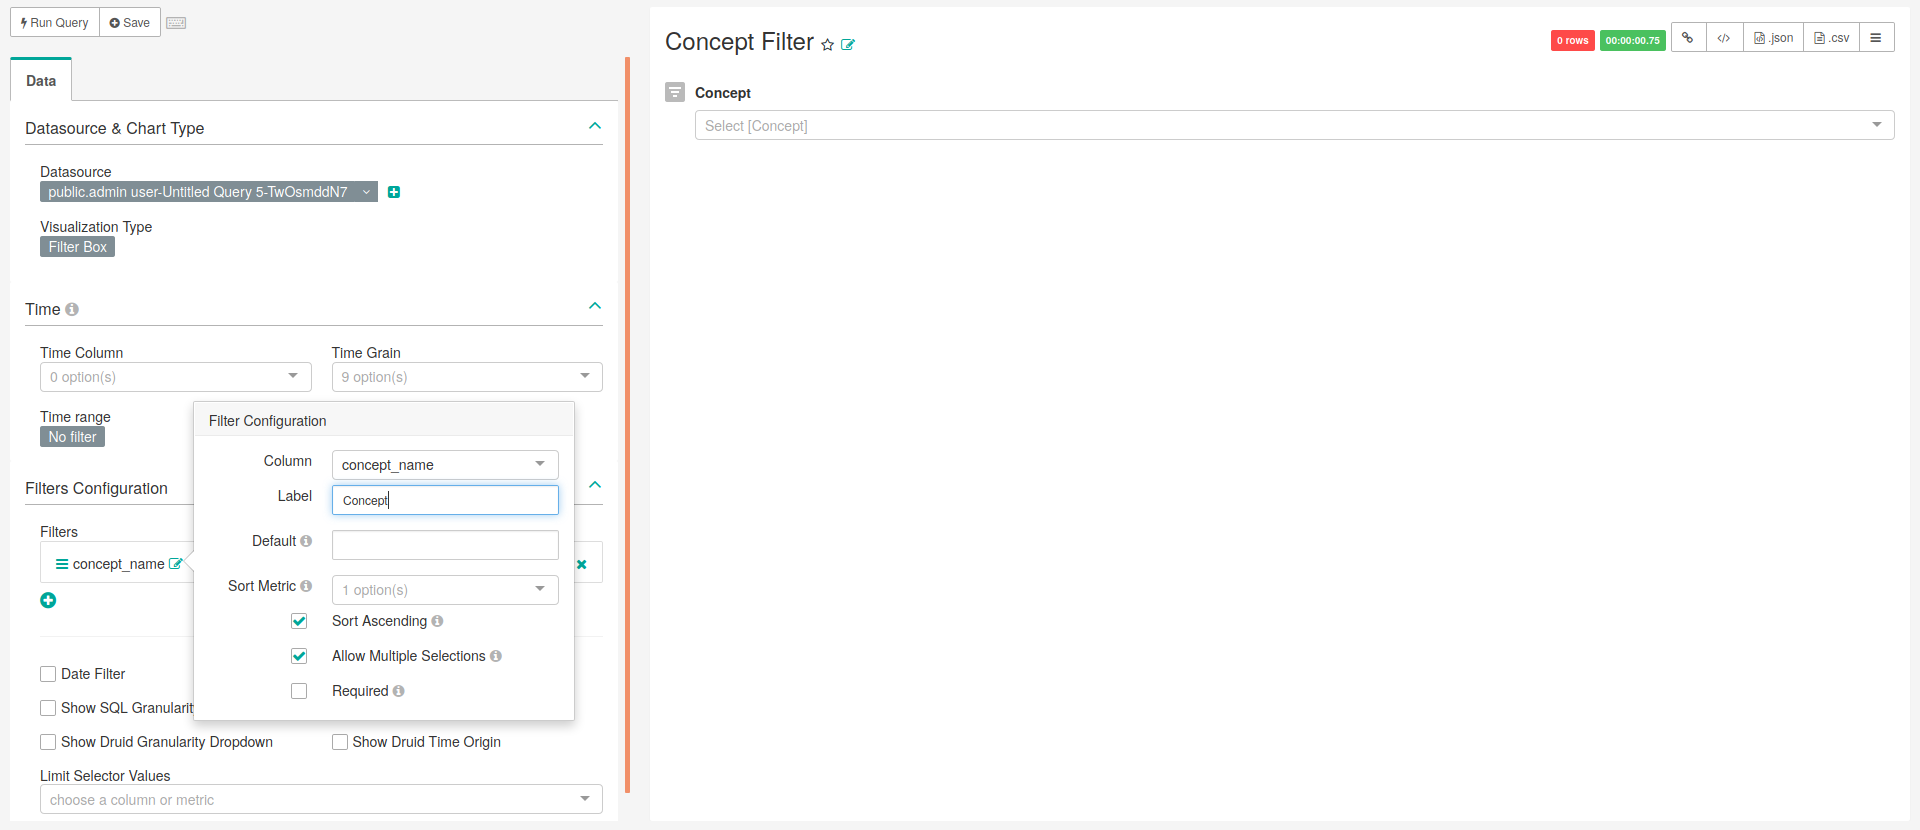
\includegraphics[width=1\linewidth]{images/conceptFilter} \caption{Settings for creating the concept filter.}\label{fig:conceptFilter}
\end{figure}

\subsubsection{Number of Concepts}\label{number-of-concepts}

Discuss what is important to see in this chart\ldots{} TO DO The main
characteristics of this chart are presented in Figure
\ref{fig:visitTypes}, being the following:

\begin{itemize}
\tightlist
\item
  \textbf{Data Tab}:

  \begin{itemize}
  \tightlist
  \item
    \textbf{Visualization Type}: Bar Chart
  \item
    \textbf{Time range}: No filter
  \item
    \textbf{Metrics}:
  \item
    \textbf{Filters}: Empty
  \item
    \textbf{Series}:
  \item
    \textbf{Breakdowns}:
  \item
    \textbf{Row limit}: Empty
  \item
    \textbf{Contribution}: Not checked
  \end{itemize}
\item
  \textbf{Costumize Tab}:

  \begin{itemize}
  \tightlist
  \item
    \textbf{Y Axis Label}:
  \item
    \textbf{X Axis Label}:
  \item
    \textbf{Legend}: Checked
  \item
    \textbf{Stacked Bars}:
  \item
    \textbf{Bar Values}:
  \item
    \textbf{Sort Bars}:
  \item
    \textbf{Extra Controls}:
  \item
    \textbf{Reduce X ticks}:
  \end{itemize}
\end{itemize}

\begin{figure}
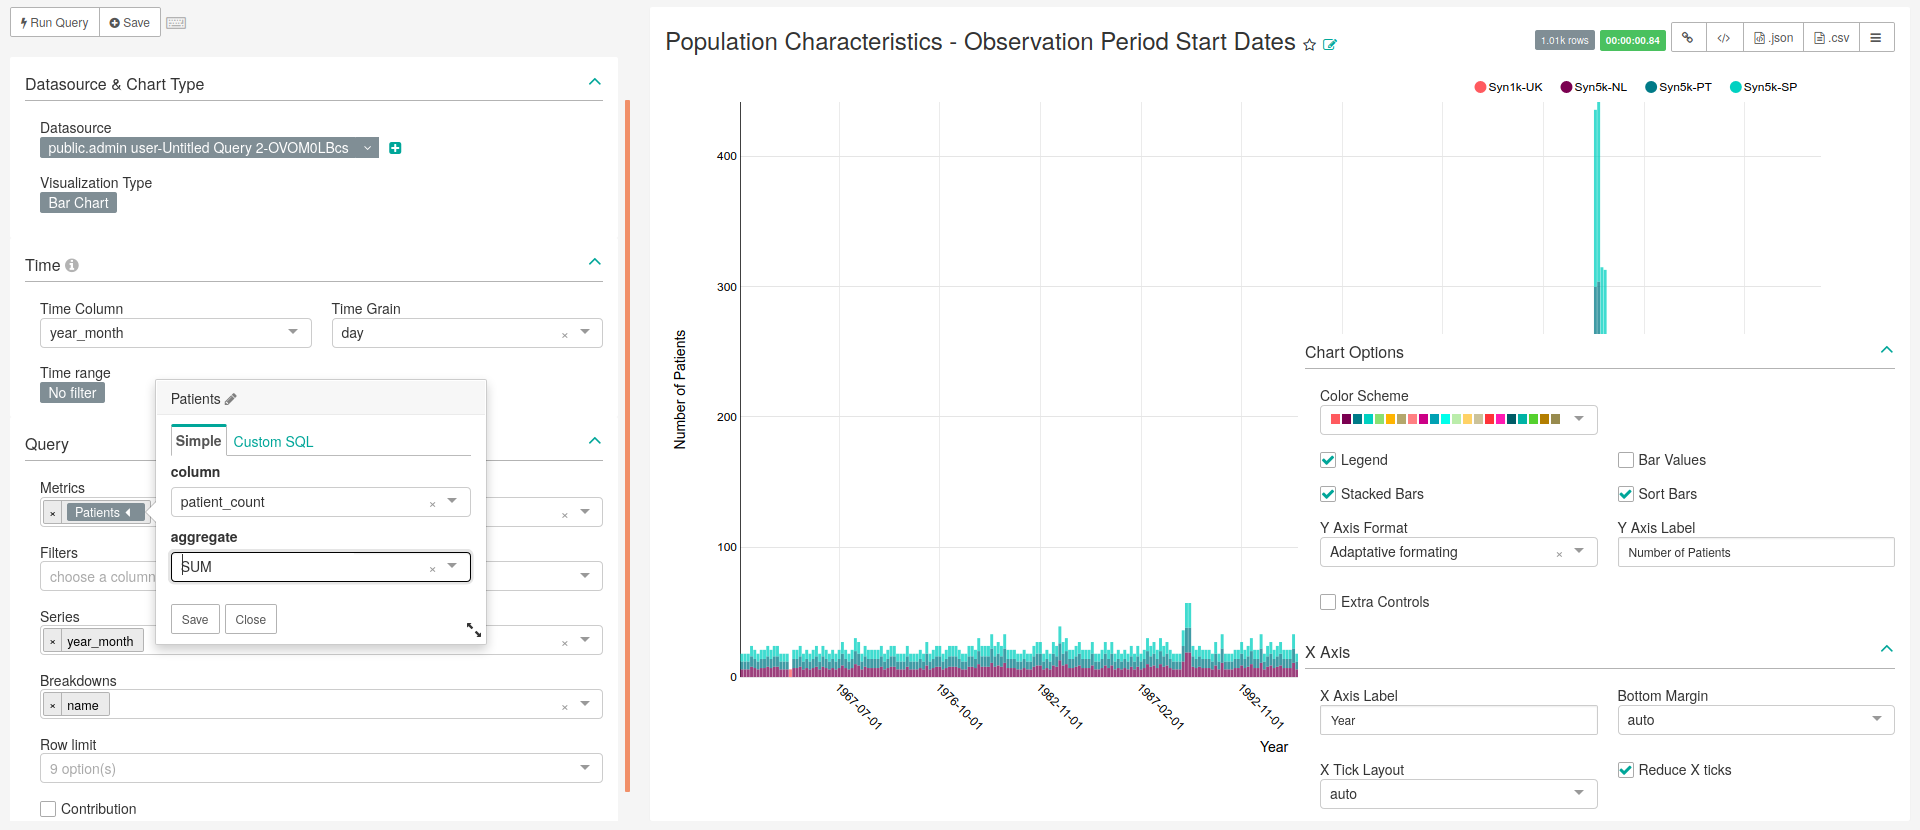
\includegraphics[width=1\linewidth]{images/populationCharacteristicsObservationPeriodStartDates} \caption{Settings for creating chart representing the number of patients at the start of their observation period (bar chart). Image changed to contain information hidden in the customize menu.}\label{fig:visitTypes8}
\end{figure}

\subsubsection{Concept Browser Table}\label{concept-browser-table}

The main characteristics of this chart are presented in Figure
\ref{fig:visitTypes}, being the following:

\begin{itemize}
\tightlist
\item
  \textbf{Data Tab}:

  \begin{itemize}
  \tightlist
  \item
    \textbf{Visualization Type}: Bar Chart
  \item
    \textbf{Time range}: No filter
  \item
    \textbf{Metrics}:
  \item
    \textbf{Filters}: Empty
  \item
    \textbf{Series}:
  \item
    \textbf{Breakdowns}:
  \item
    \textbf{Row limit}: Empty
  \item
    \textbf{Contribution}: Not checked
  \end{itemize}
\item
  \textbf{Costumize Tab}:

  \begin{itemize}
  \tightlist
  \item
    \textbf{Y Axis Label}:
  \item
    \textbf{X Axis Label}:
  \item
    \textbf{Legend}: Checked
  \item
    \textbf{Stacked Bars}:
  \item
    \textbf{Bar Values}:
  \item
    \textbf{Sort Bars}:
  \item
    \textbf{Extra Controls}:
  \item
    \textbf{Reduce X ticks}:
  \end{itemize}
\end{itemize}

\begin{figure}
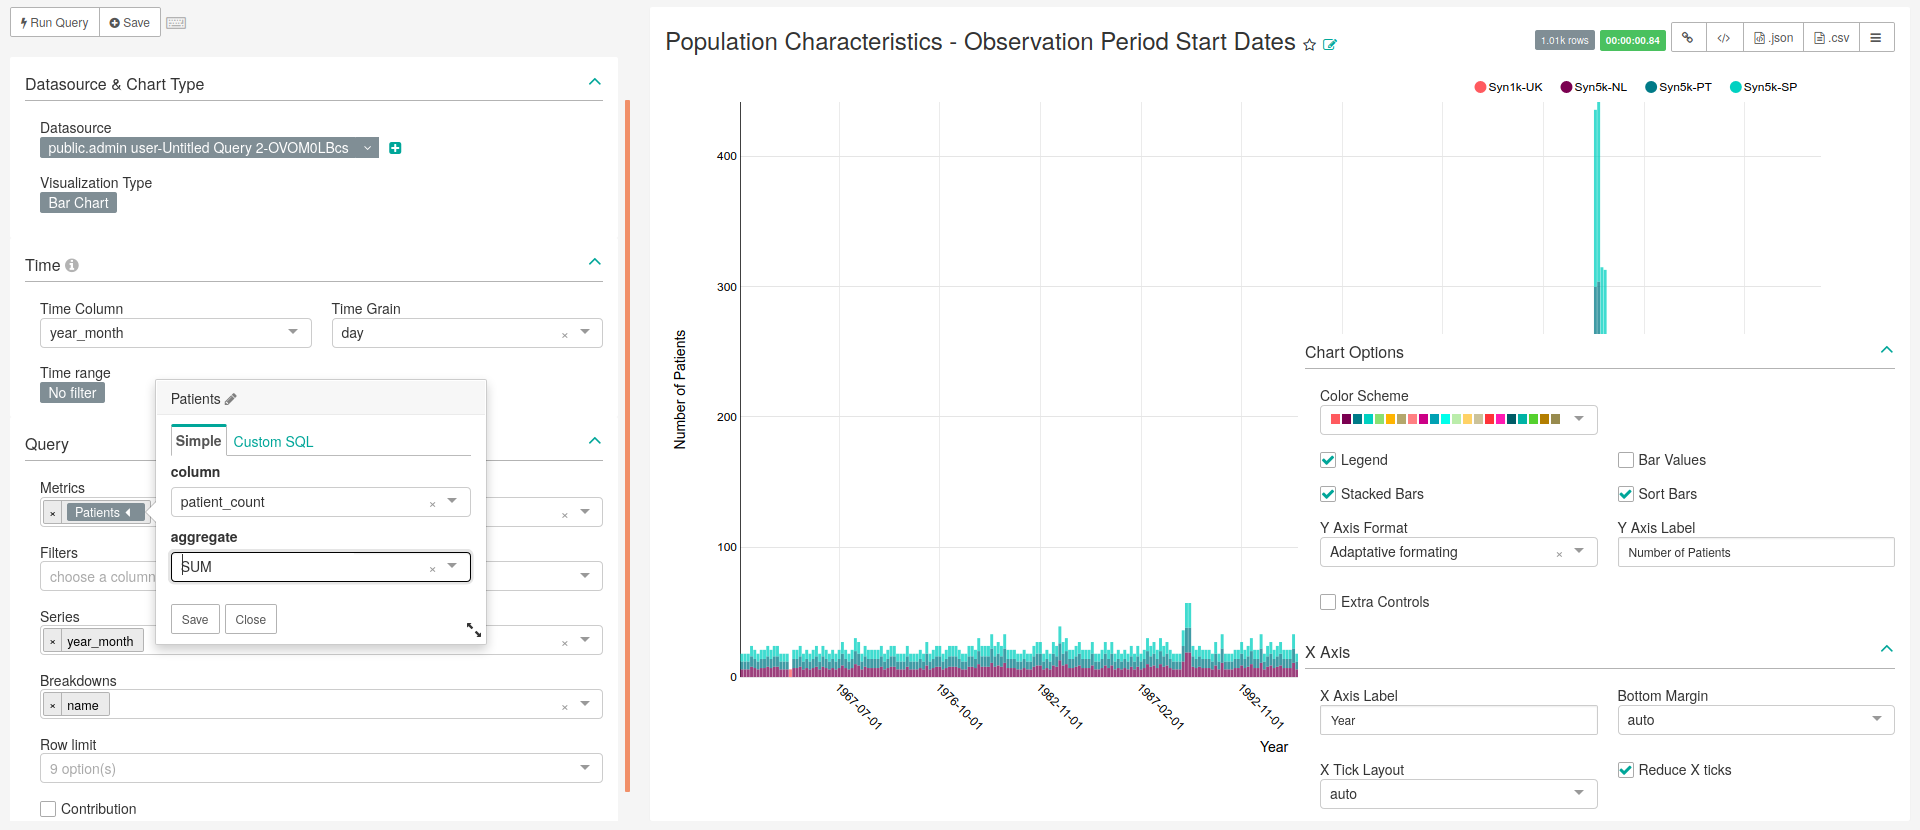
\includegraphics[width=1\linewidth]{images/populationCharacteristicsObservationPeriodStartDates} \caption{Settings for creating chart representing the number of patients at the start of their observation period (bar chart). Image changed to contain information hidden in the customize menu.}\label{fig:visitTypes3}
\end{figure}

\subsubsection{\# of Occurrences}\label{of-occurrences}

The main characteristics of this chart are presented in Figure
\ref{fig:visitTypes}, being the following:

\begin{itemize}
\tightlist
\item
  \textbf{Data Tab}:

  \begin{itemize}
  \tightlist
  \item
    \textbf{Visualization Type}: Bar Chart
  \item
    \textbf{Time range}: No filter
  \item
    \textbf{Metrics}:
  \item
    \textbf{Filters}: Empty
  \item
    \textbf{Series}:
  \item
    \textbf{Breakdowns}:
  \item
    \textbf{Row limit}: Empty
  \item
    \textbf{Contribution}: Not checked
  \end{itemize}
\item
  \textbf{Costumize Tab}:

  \begin{itemize}
  \tightlist
  \item
    \textbf{Y Axis Label}:
  \item
    \textbf{X Axis Label}:
  \item
    \textbf{Legend}: Checked
  \item
    \textbf{Stacked Bars}:
  \item
    \textbf{Bar Values}:
  \item
    \textbf{Sort Bars}:
  \item
    \textbf{Extra Controls}:
  \item
    \textbf{Reduce X ticks}:
  \end{itemize}
\end{itemize}

\begin{figure}
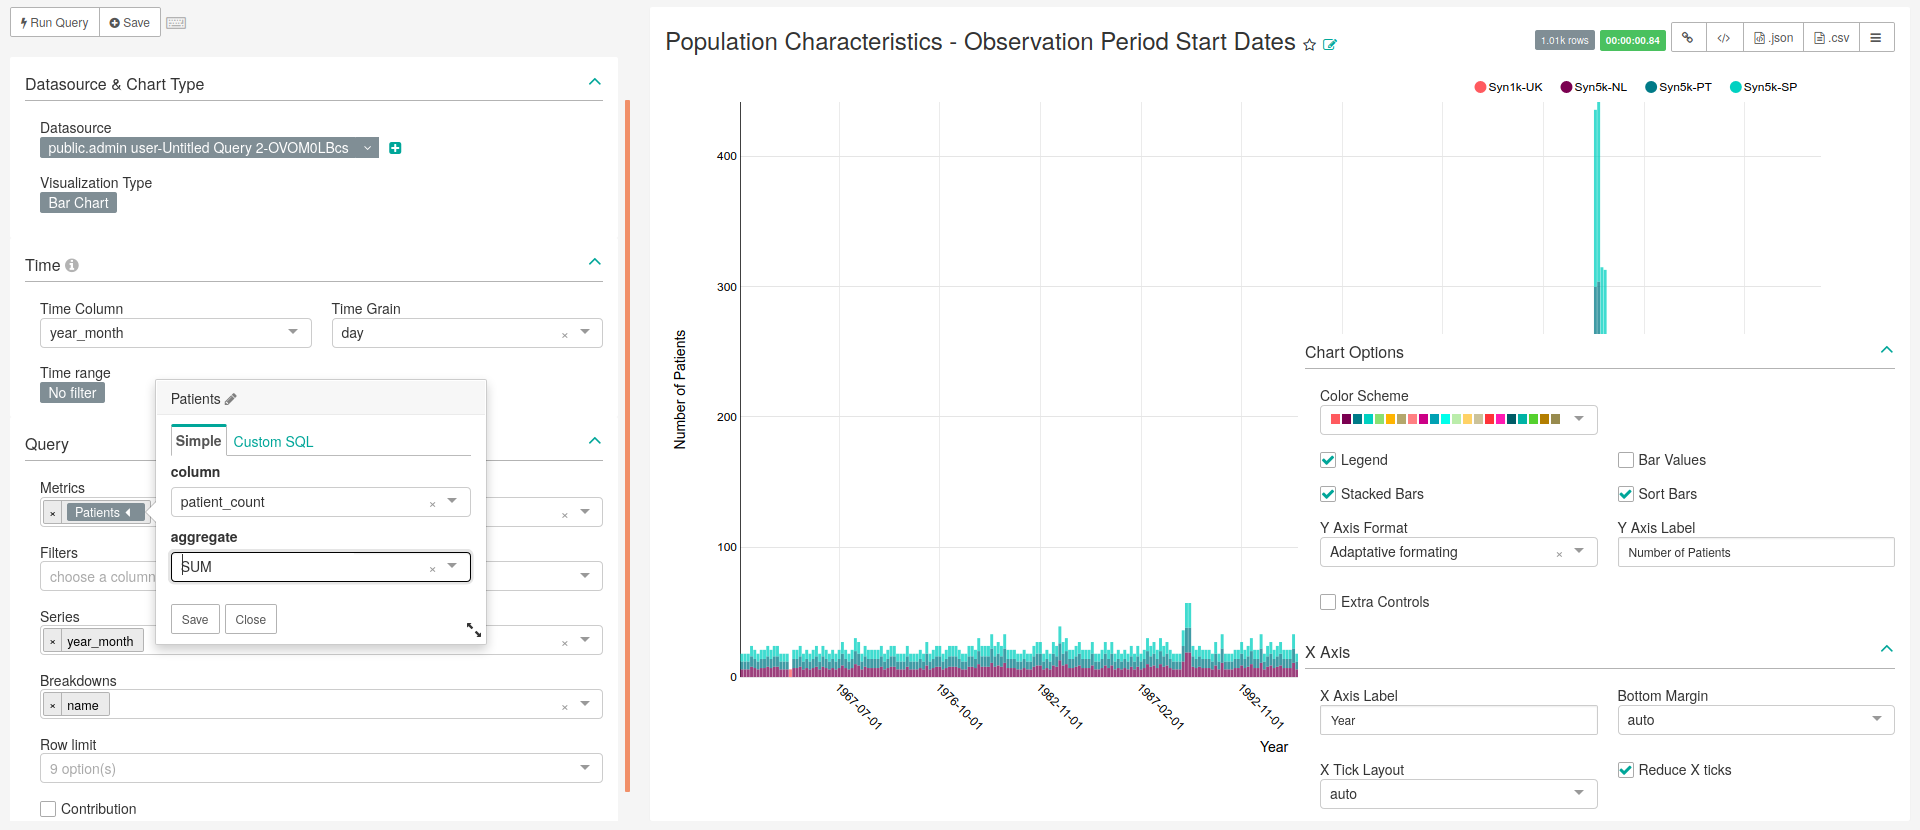
\includegraphics[width=1\linewidth]{images/populationCharacteristicsObservationPeriodStartDates} \caption{Settings for creating chart representing the number of patients at the start of their observation period (bar chart). Image changed to contain information hidden in the customize menu.}\label{fig:visitTypes4}
\end{figure}

\subsubsection{\# of Patients}\label{of-patients}

The main characteristics of this chart are presented in Figure
\ref{fig:visitTypes}, being the following:

\begin{itemize}
\tightlist
\item
  \textbf{Data Tab}:

  \begin{itemize}
  \tightlist
  \item
    \textbf{Visualization Type}: Bar Chart
  \item
    \textbf{Time range}: No filter
  \item
    \textbf{Metrics}:
  \item
    \textbf{Filters}: Empty
  \item
    \textbf{Series}:
  \item
    \textbf{Breakdowns}:
  \item
    \textbf{Row limit}: Empty
  \item
    \textbf{Contribution}: Not checked
  \end{itemize}
\item
  \textbf{Costumize Tab}:

  \begin{itemize}
  \tightlist
  \item
    \textbf{Y Axis Label}:
  \item
    \textbf{X Axis Label}:
  \item
    \textbf{Legend}: Checked
  \item
    \textbf{Stacked Bars}:
  \item
    \textbf{Bar Values}:
  \item
    \textbf{Sort Bars}:
  \item
    \textbf{Extra Controls}:
  \item
    \textbf{Reduce X ticks}:
  \end{itemize}
\end{itemize}

\begin{figure}
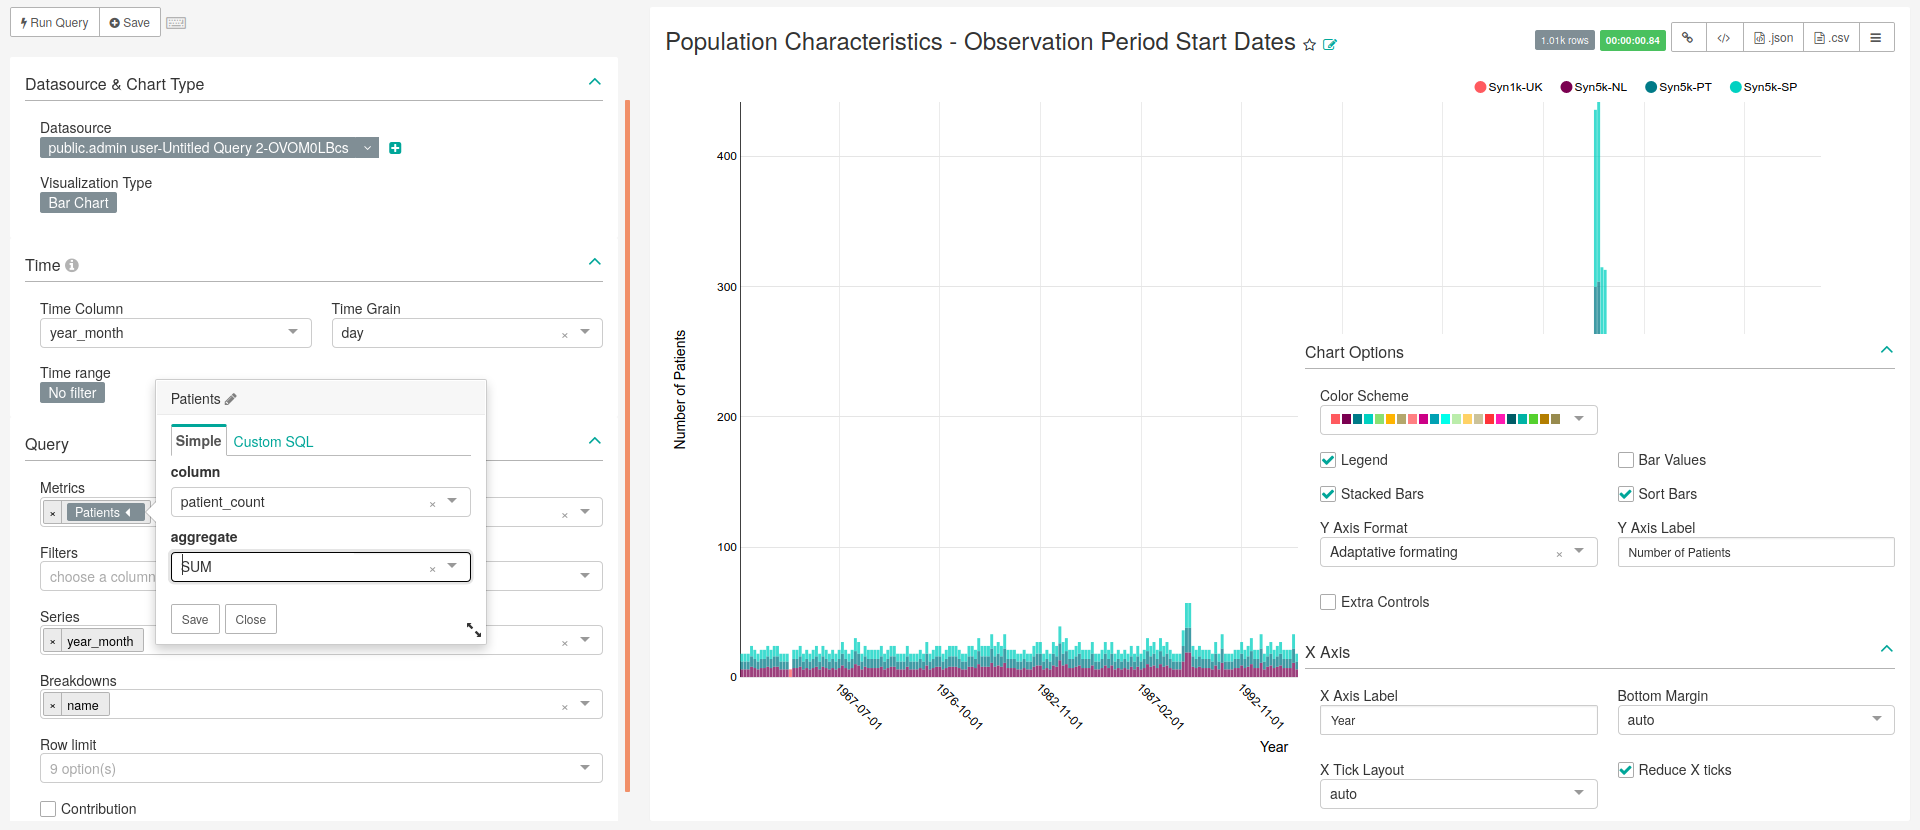
\includegraphics[width=1\linewidth]{images/populationCharacteristicsObservationPeriodStartDates} \caption{Settings for creating chart representing the number of patients at the start of their observation period (bar chart). Image changed to contain information hidden in the customize menu.}\label{fig:visitTypes5}
\end{figure}

\section{Concepts Domains Tab}\label{concepts-domains-tab}

This tab is composed of six bar charts that show the percentage of
existent concepts in each database. These charts are similar but divided
by the concept domains existent in the standard vocabularies, which are
the conditions, procedures, drugs, observations, measurements and
devices. Figure \ref{fig:conceptsDomainsLayout} shows this dashboard's
layout.

\begin{figure}
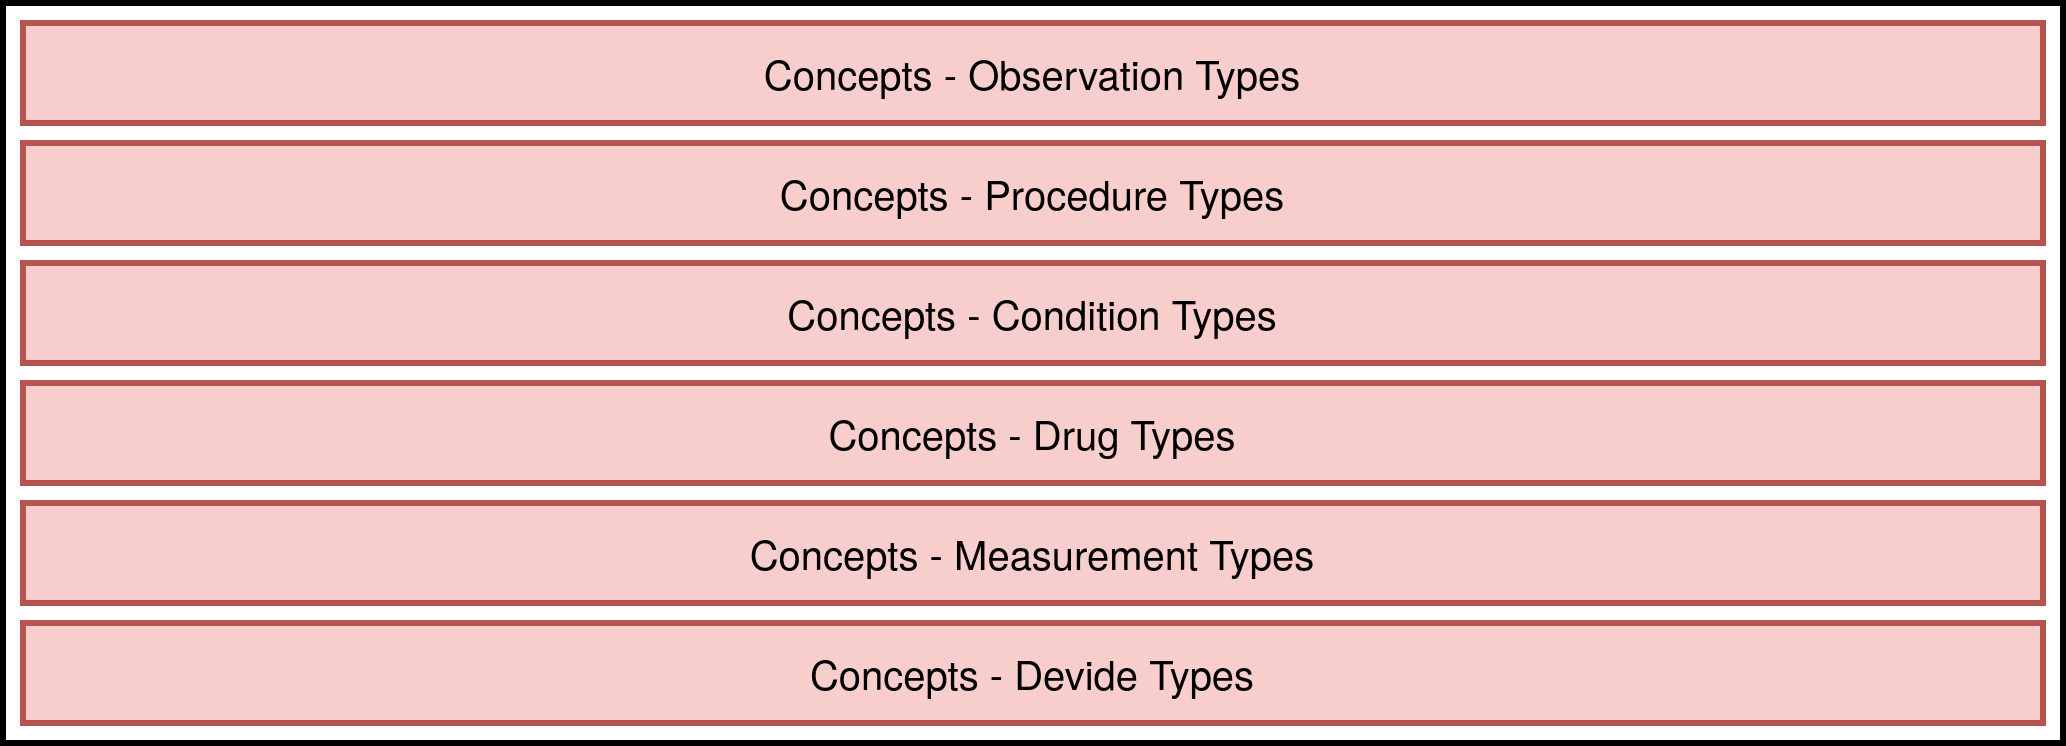
\includegraphics[width=1\linewidth]{images/conceptsDomainsLayout} \caption{Distribution of charts on the dashboard.}\label{fig:conceptsDomainsLayout}
\end{figure}

\subsection{SQL query}\label{sql-query-17}

\begin{Shaded}
\begin{Highlighting}[]
\CommentTok{-- Concepts Domains}
\KeywordTok{SELECT}\NormalTok{ source.name,}
    \KeywordTok{CASE} \KeywordTok{WHEN}\NormalTok{ analysis_id = }\DecValTok{405} \KeywordTok{THEN} \StringTok{'Condition'}
    \KeywordTok{WHEN}\NormalTok{ analysis_id = }\DecValTok{605} \KeywordTok{THEN} \StringTok{'Procedure'}
    \KeywordTok{WHEN}\NormalTok{ analysis_id = }\DecValTok{705} \KeywordTok{THEN} \StringTok{'Drug'}
    \KeywordTok{WHEN}\NormalTok{ analysis_id = }\DecValTok{805} \KeywordTok{THEN} \StringTok{'Observation'}
    \KeywordTok{WHEN}\NormalTok{ analysis_id = }\DecValTok{1805} \KeywordTok{THEN} \StringTok{'Measurement'}
    \KeywordTok{WHEN}\NormalTok{ analysis_id = }\DecValTok{2105} \KeywordTok{THEN} \StringTok{'Device'}
    \KeywordTok{ELSE} \StringTok{'Other'} \KeywordTok{END} \KeywordTok{AS}\NormalTok{ domain_name,}
\NormalTok{    concept_name, }\FunctionTok{sum}\NormalTok{(count_value) }\KeywordTok{AS}\NormalTok{ num_records}
\KeywordTok{FROM}\NormalTok{ public.achilles_results }\KeywordTok{AS}\NormalTok{ achilles }
    \KeywordTok{INNER} \KeywordTok{JOIN}\NormalTok{ public.data_source }\KeywordTok{AS} \KeywordTok{source} \KeywordTok{ON} 
\NormalTok{      achilles.data_source_id=source.id}
    \KeywordTok{INNER} \KeywordTok{JOIN}\NormalTok{ public.concept }\KeywordTok{AS}\NormalTok{ c1 }\KeywordTok{ON} 
\NormalTok{      stratum_2 = }\FunctionTok{CAST}\NormalTok{(concept_id }\KeywordTok{AS}\NormalTok{ text)}
\KeywordTok{WHERE}\NormalTok{ analysis_id }\KeywordTok{IN}\NormalTok{ (}\DecValTok{405}\NormalTok{, }\DecValTok{605}\NormalTok{, }\DecValTok{705}\NormalTok{, }\DecValTok{805}\NormalTok{, }\DecValTok{1805}\NormalTok{, }\DecValTok{2105}\NormalTok{)}
\KeywordTok{GROUP} \KeywordTok{BY}\NormalTok{ source.name, concept_name, }
    \KeywordTok{CASE} \KeywordTok{WHEN}\NormalTok{ analysis_id = }\DecValTok{405} \KeywordTok{THEN} \StringTok{'Condition'}
    \KeywordTok{WHEN}\NormalTok{ analysis_id = }\DecValTok{605} \KeywordTok{THEN} \StringTok{'Procedure'}
    \KeywordTok{WHEN}\NormalTok{ analysis_id = }\DecValTok{705} \KeywordTok{THEN} \StringTok{'Drug'}
    \KeywordTok{WHEN}\NormalTok{ analysis_id = }\DecValTok{805} \KeywordTok{THEN} \StringTok{'Observation'}
    \KeywordTok{WHEN}\NormalTok{ analysis_id = }\DecValTok{1805} \KeywordTok{THEN} \StringTok{'Measurement'}
    \KeywordTok{WHEN}\NormalTok{ analysis_id = }\DecValTok{2105} \KeywordTok{THEN} \StringTok{'Device'}
    \KeywordTok{ELSE} \StringTok{'Other'} \KeywordTok{END}
\end{Highlighting}
\end{Shaded}

\subsection{Chart settings}\label{chart-settings-16}

The difference between the six charts related to concept domains is the
condition in the filter. Therefore, to create all the charts of this
dashboard, it is necessary to follow the main characteristics presented
in Figure \ref{fig:conceptsDomainTypes} and the list of possible values
for the filter. Those characteristics are the following:

\begin{itemize}
\tightlist
\item
  \textbf{Data Tab}:

  \begin{itemize}
  \tightlist
  \item
    \textbf{Visualization Type}: Bar Chart
  \item
    \textbf{Time range}: No filter
  \item
    \textbf{Metrics}: SUM(num\_records) as ``Nr Records''
  \item
    \textbf{Filters}: domain = \textbf{See filter list}
  \item
    \textbf{Series}: name
  \item
    \textbf{Breakdowns}: concept\_name
  \item
    \textbf{Row limit}: Empty
  \item
    \textbf{Contribution}: Checked
  \end{itemize}
\item
  \textbf{Costumize Tab}:

  \begin{itemize}
  \tightlist
  \item
    \textbf{Y Axis Label}:
  \item
    \textbf{X Axis Label}:
  \item
    \textbf{Legend}: Checked
  \item
    \textbf{Stacked Bars}: Checked
  \item
    \textbf{Bar Values}: Not checked
  \item
    \textbf{Sort Bars}: Not checked
  \item
    \textbf{Extra Controls}: Not checked
  \item
    \textbf{Reduce X ticks}: Not checked
  \end{itemize}
\item
  \textbf{Filter List}:

  \begin{itemize}
  \tightlist
  \item
    \textbf{Concepts - Condition Types}: Condition
  \item
    \textbf{Concepts - Procedure Types}: Procedure
  \item
    \textbf{Concepts - Drug Types}: Drug
  \item
    \textbf{Concepts - Observation Types}: Observation
  \item
    \textbf{Concepts - Measurement Types}: Measurement
  \item
    \textbf{Concepts - Device Types}: Device
  \end{itemize}
\end{itemize}

\begin{figure}
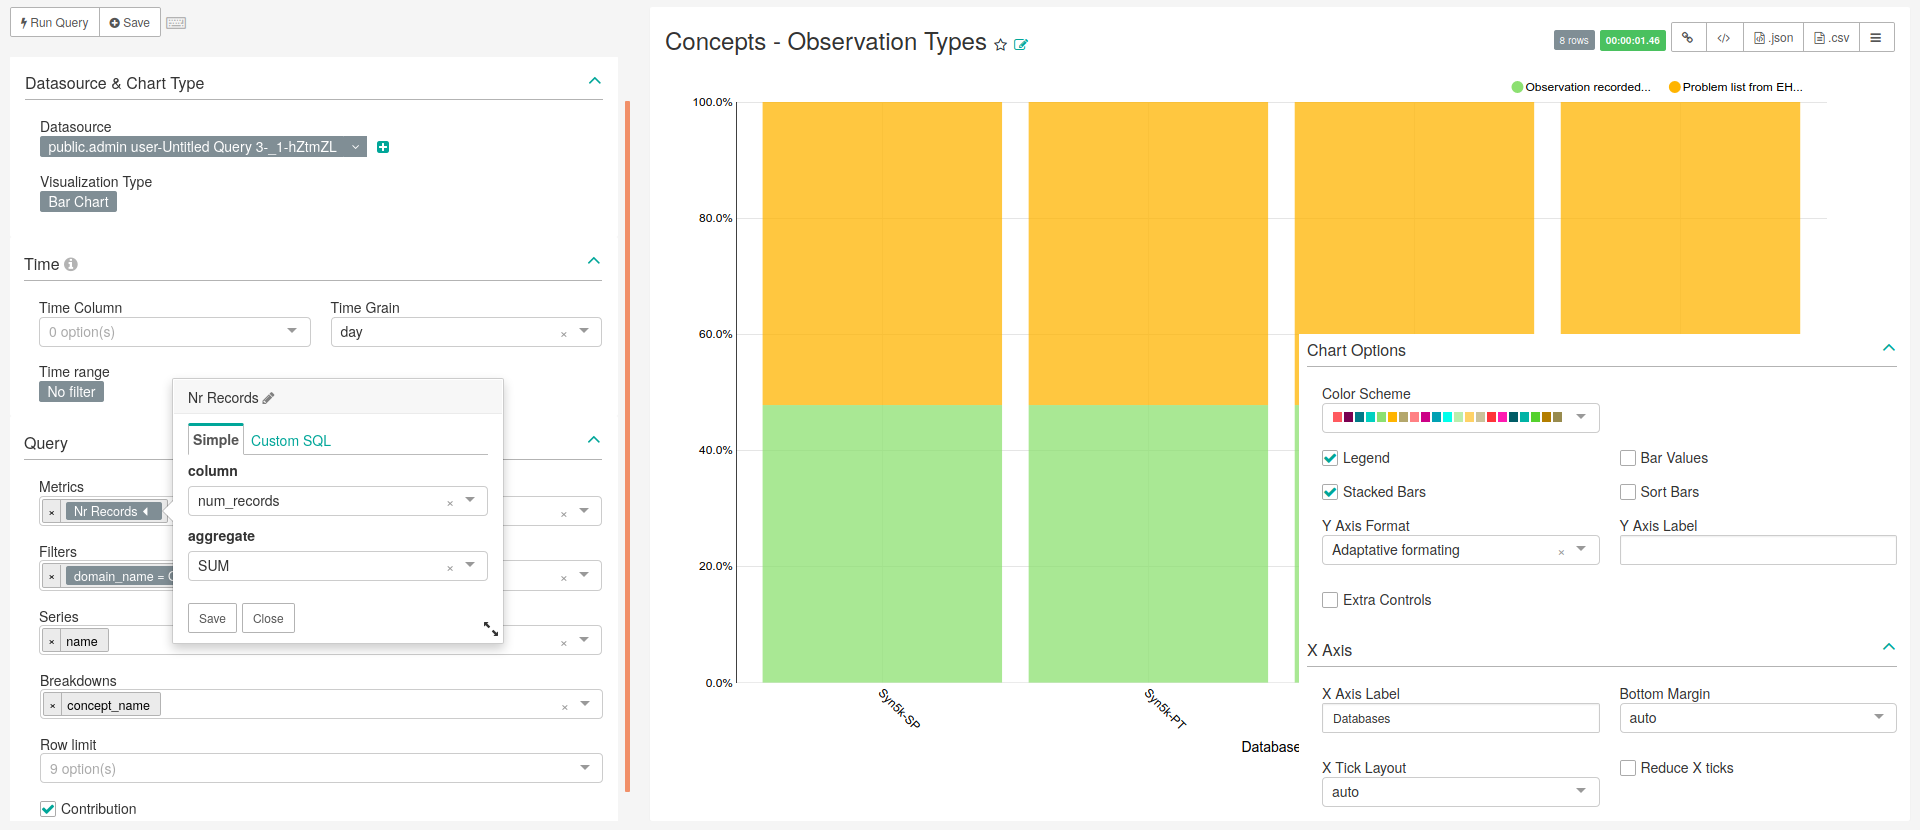
\includegraphics[width=1\linewidth]{images/conceptsDomainTypes} \caption{Settings for creating all the charts related with the concept domains for each databases (bar chart). Image changed to contain information hidden in the customize menu.}\label{fig:conceptsDomainTypes}
\end{figure}

\chapter{Data Domains}\label{data-domains}

In this dashboard is present the `'Database Type Filter'', that was
detailed in the Chapter General.

\section{Data Domains - Number of Records per
Peson}\label{data-domains---number-of-records-per-peson}

\subsection{SQL query}\label{sql-query-18}

\begin{Shaded}
\begin{Highlighting}[]
\CommentTok{-- 201, 401, 501, 601, 701, 801, 1801, 2101, 2201   }
\CommentTok{-- Data domains - Number of records per peson}
\KeywordTok{SELECT} 
\NormalTok{    source.name,}
    \KeywordTok{CASE} 
      \KeywordTok{WHEN}\NormalTok{ analysis_id = }\DecValTok{201} \KeywordTok{THEN} \StringTok{'Visit'}
      \KeywordTok{WHEN}\NormalTok{ analysis_id = }\DecValTok{401} \KeywordTok{THEN} \StringTok{'Condition'}
      \KeywordTok{WHEN}\NormalTok{ analysis_id = }\DecValTok{501} \KeywordTok{THEN} \StringTok{'Death'}
      \KeywordTok{WHEN}\NormalTok{ analysis_id = }\DecValTok{601} \KeywordTok{THEN} \StringTok{'Procedure'}
      \KeywordTok{WHEN}\NormalTok{ analysis_id = }\DecValTok{701} \KeywordTok{THEN} \StringTok{'Drug Exposure'}
      \KeywordTok{WHEN}\NormalTok{ analysis_id = }\DecValTok{801} \KeywordTok{THEN} \StringTok{'Observation'}
      \KeywordTok{WHEN}\NormalTok{ analysis_id = }\DecValTok{1801} \KeywordTok{THEN} \StringTok{'Measurement'}
      \KeywordTok{WHEN}\NormalTok{ analysis_id = }\DecValTok{2101} \KeywordTok{THEN} \StringTok{'Device'}
      \KeywordTok{WHEN}\NormalTok{ analysis_id = }\DecValTok{2201} \KeywordTok{THEN} \StringTok{'Note'}
    \KeywordTok{END} \KeywordTok{AS}\NormalTok{ Data_Domain,}
    \FunctionTok{SUM}\NormalTok{(count_value) /AVG(num_persons) }\KeywordTok{AS} \OtherTok{"Records per person"}\NormalTok{,}
\NormalTok{    source.slug}
\KeywordTok{FROM}\NormalTok{ public.achilles_results }\KeywordTok{AS}\NormalTok{ achilles }
    \KeywordTok{INNER} \KeywordTok{JOIN}\NormalTok{ public.data_source }\KeywordTok{AS} \KeywordTok{source} \KeywordTok{ON} 
\NormalTok{      achilles.data_source_id=source.id}
    \KeywordTok{INNER} \KeywordTok{JOIN}\NormalTok{ (}
        \KeywordTok{SELECT}\NormalTok{ data_source_id , count_value }\KeywordTok{AS}\NormalTok{ num_persons }
        \KeywordTok{FROM}\NormalTok{ achilles_results }
        \KeywordTok{WHERE}\NormalTok{ analysis_id = }\DecValTok{1}
\NormalTok{        ) counts }\KeywordTok{ON} 
\NormalTok{      achilles.data_source_id = counts.data_source_id }
\KeywordTok{GROUP} \KeywordTok{BY}\NormalTok{ analysis_id, source.name, source.slug}
\KeywordTok{HAVING}\NormalTok{ analysis_id }\KeywordTok{IN}\NormalTok{ (}\DecValTok{201}\NormalTok{, }\DecValTok{401}\NormalTok{, }\DecValTok{501}\NormalTok{, }\DecValTok{601}\NormalTok{, }\DecValTok{701}\NormalTok{, }\DecValTok{801}\NormalTok{, }\DecValTok{1801}\NormalTok{, }\DecValTok{2101}\NormalTok{, }
    \DecValTok{2201}\NormalTok{)}
\end{Highlighting}
\end{Shaded}

\subsection{Chart settings}\label{chart-settings-17}

The main characteristics of this chart are presented in Figure
\ref{fig:dataDomainsNumberOfRecordsPerPeson}, being the following:

\begin{itemize}
\tightlist
\item
  \textbf{Data Tab}:

  \begin{itemize}
  \tightlist
  \item
    \textbf{Visualization Type}: Heatmap
  \item
    \textbf{Time range}: No filter
  \item
    \textbf{X}: name
  \item
    \textbf{Y}: data\_domain
  \item
    \textbf{Metric}: SUM(records\_per\_person) as ``Sum of records per
    person''
  \item
    \textbf{Filters}: Empty
  \item
    \textbf{Row limit}: Empty
  \item
    \textbf{Legend}: Checked
  \item
    \textbf{Show percentage}: Checked
  \item
    \textbf{Show Values}: Not checked
  \item
    \textbf{Normalized}: Not checked
  \end{itemize}
\end{itemize}

\begin{figure}
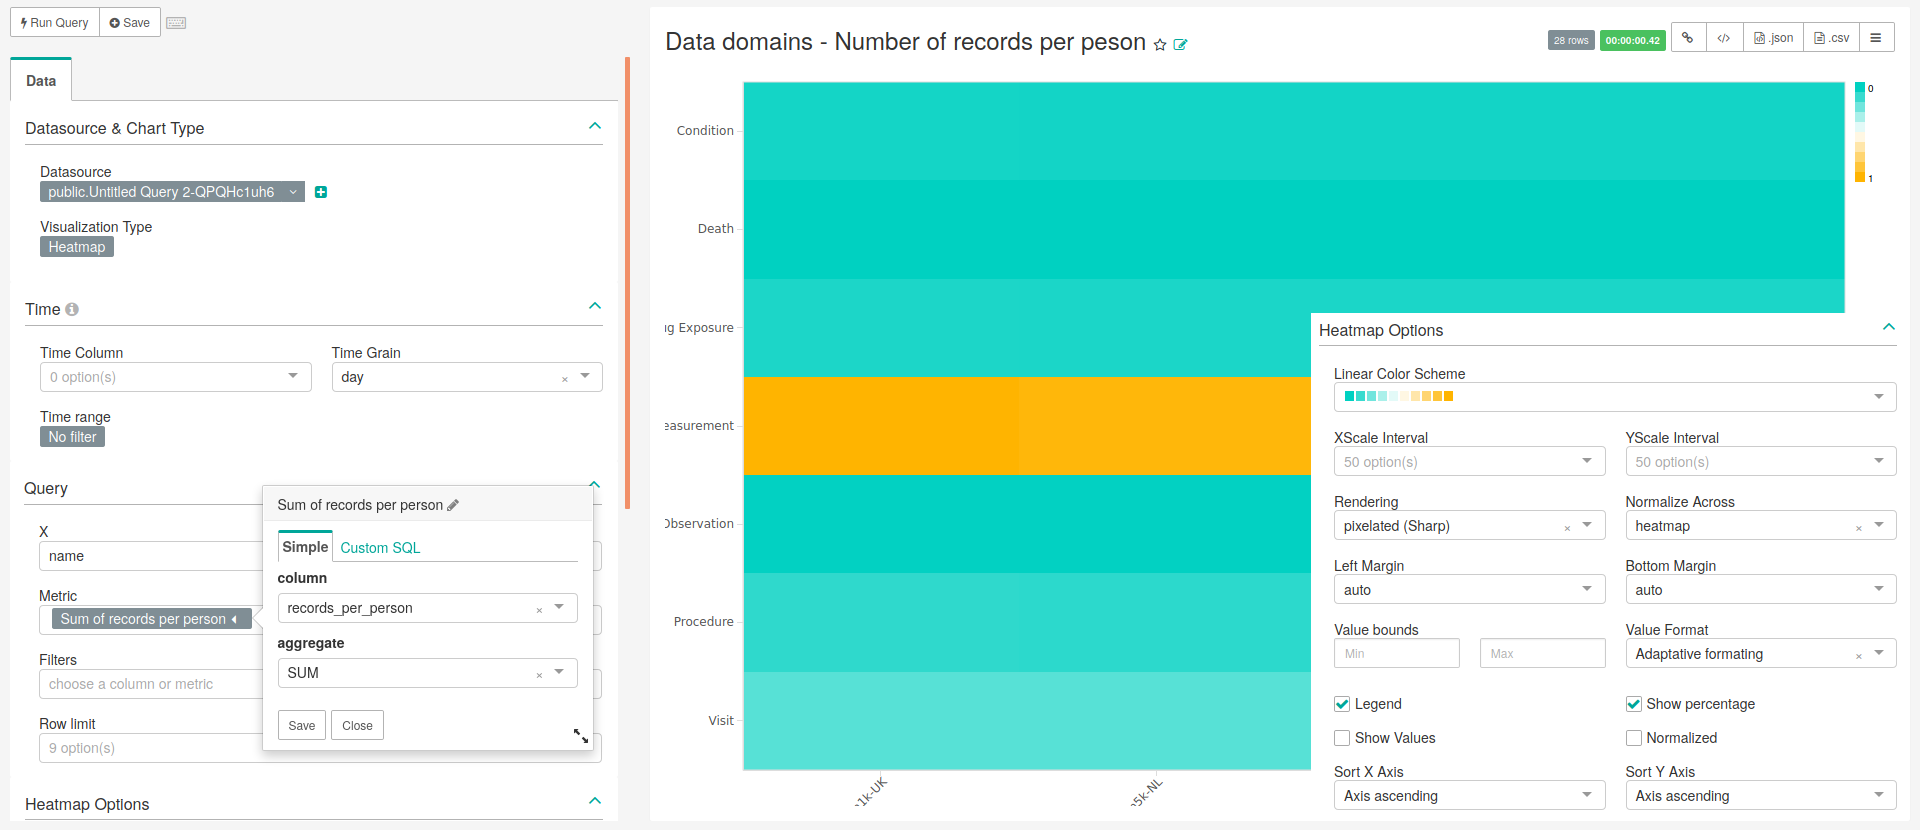
\includegraphics[width=1\linewidth]{images/dataDomainsNumberOfRecordsPerPeson} \caption{Settings for creating chart representing the number of records per patient in the different data domains (heatmap). Image changed to contain information hidden in the customize menu.}\label{fig:dataDomainsNumberOfRecordsPerPeson}
\end{figure}

\bibliography{refs.bib}

\end{document}
